\documentclass[final]{siamltex}


\title{The cutoff phenomenon and mixing by chaotic maps}

\author{T. Liang\thanks{Department of Aeronautics and Astronautics,
    Stanford University, Stanford, CA 94305, USA ({\tt
      hartree50@gmail.com}).}  \and M. West\thanks{Department of
    Mechanical Science and Engineering, University of Illinois at
    Urbana-Champaign, Urbana, IL 61801, USA ({\tt
      mwest@illinois.edu}).}}






%\documentclass{article}

%\usepackage{graphicx,psfrag}
\usepackage{graphicx}
%\usepackage{graphics}
\usepackage{amsmath}
%\usepackage{amsthm}
%\usepackage{amsfonts}
\usepackage{amssymb}
%\usepackage[margin=3cm]{geometry}
%\usepackage{hyperref}

%\title{The Cutoff Phenomenon and \\Mixing by Chaotic Maps}
%\author{Tzu-Chen Liang and Matthew West}
%\date{\today}
\graphicspath{{figures/}}
% End of Preamble


%\newtheorem{assumption}{Assumption}
%\newtheorem{definition}{Definition}
%\newtheorem{theorem}{Theorem}
%\newtheorem{lemma}{Lemma}
\newtheorem{example_base}{Example}
\newenvironment{example}{\begin{example_base}}
   {\hspace{\stretch{1}}$\lozenge$\end{example_base}}

%\newtheorem{proof_base}{Proof}
%\newenvironment{proof}{\begin{proof_base}}
%   {\hspace{\stretch{1}}$\blacksquare$\end{proof_base}}


\DeclareMathOperator{\erf}{erf}
\DeclareMathOperator{\prob}{Prob}

\usepackage{color}
\newcommand{\todo}[1]{\noindent\framebox{\begin{minipage}{0.97\columnwidth}\color{red}#1\end{minipage}}}

% disable ToDo boxes
%\renewcommand{\todo}[1]{}

\begin{document}
\maketitle
%%%%%%%%%%%%%%%%%%%%%%%%%%%%%%%%%%%%%%%%%%%%%%%%%%%%%%%%%%
%%%%%%%%%%%%%%%%%%%%%%%%%%%%%%%%%%%%%%%%%%%%%%%%%%%%%%%%%%
\begin{abstract}
  We extend the definition of a cutoff from finite Markov chains to
  the evolution of probability distributions by the Perron-Frobenius
  operator of 1D maps. We prove that if the map has full shift
  symbolic dynamics then, for appropriately chosen initial
  distributions, such an evolution exhibits a total variation
  cutoff. Moreover, the initial distributions can be chosen so that
  the limiting evolution has the same normal shape as is found in many
  Markov chain problems.
\end{abstract}


\begin{keywords} 
Cutoff phenomenon, chaotic mixing, symbolic dynamics.
\end{keywords}

\begin{AMS}
37A25, 60J05, 37B10
\end{AMS}

% 37A25   	Ergodicity, mixing, rates of mixing
% 37B10   	Symbolic dynamics
% 37E05   	Maps of the interval
% 60J05   	Discrete-time Markov processes on general state spaces

\pagestyle{myheadings}
\thispagestyle{plain}
\markboth{T. LIANG AND M. WEST}{CUTOFFS AND CHAOTIC MIXING}


%%%%%%%%%%%%%%%%%%%%%%%%%%%%%%%%%%%%%%%%%%%%%%%%%%%%%%%%%%
%%%%%%%%%%%%%%%%%%%%%%%%%%%%%%%%%%%%%%%%%%%%%%%%%%%%%%%%%%
\section{Introduction}
\label{sec:symdynintro}

\subsection{Cutoff phenomenon}
How many riffle shuffles are required to adequately mix 52 cards?
This question has been answered by Bayer and
Diaconis~\cite{Diaconis1992}. It is quite surprising that the cards
are highly ordered for the first several shuffles (up to 6 shuffles
for 52 cards) and then become randomized almost abruptly.  This kind
of sharp change in some measure of order has been discovered in many
finite Markov Chains, and is termed the \emph{cutoff
  phenomenon}~\cite{Diaconis1986}. A good review of the cutoff
phenomenon for random walks on finite groups has been given by
Saloff-Coste~\cite{LSaloff-Costt2004}.

In general, proving the
existence of a cutoff in a certain sequence of Markov chains is a
difficult task. It usually requires some clever insight about the
system, such as the famous example of the ``rising sequence''
formulation of the riffle shuffle problem \cite{Diaconis1992}. Showing
cutoff numerically is equally difficult because it usually entails the
simulation of very large Markov chains. As a result, our knowledge
about cutoff phenomena is limited. Diaconis~\cite{Diaconis1996,
  Diaconis2005} asks, ``How widespread is the cutoff phenomenon for
families of finite ergodic Markov chains and how can one recognize
it?'' In this paper we provide a new class of systems that
exhibit cutoff phenomena using chaotic maps.

\todo{TC: I added package hyperref in the begining for quick reference. Please take it out if it's not appropriate.}

\todo{MW: add references below for ``random search strategies'' and
  ``generating random numbers''.}

\subsection{Chaotic map mixing}
In other work, the mixing process of chaotic maps or flows has been
observed to have similar multistage behavior~\cite{Thiffeault2003-13,
  Thiffeault2004, Tsang2005} to that of cutoff. Think of cream being
stirred into a cup of coffee: initially the cream is stretched and
folded, but remains distinct from the coffee, but then they rapidly
mix and become indistinguishable.  Chaotic mixing have been observed
in experiments \cite{Rothstein1999, Voth2002}, can be simulated by
large-scale computations \cite{topopt, Tsang2005}, and have been
applied in, for example, microfluidic mixing channel design
\cite{Ottino2004Science, Wiggins2004, Ottino2004}, random search
strategies and generating random numbers.

A widely observed phenomenon in the chaotic mixing process with small
diffusion is the two- or three-stage transition
\cite{Thiffeault2003-13, Fereday2002, Antonsen1996}. The map does not
mix a scalar function with a constant rate in general. When the
variance of the scalar function is measured during the mixing process,
one generally observes a relatively flat decay followed by a
super-exponential change, before it finally tends to an exponential
decay. We are interested in when these transitions happen, why they
happen, and how to predict the slope of the exponential region. A good
review and physical interpretation is given by
Thiffeault~\cite{Thiffeault2004}.

\subsection{Cutoff for chaotic maps}
In this article, we build an explicit relationship between the cutoff
phenomenon for finite Markov chains and the chaotic mixing process by
developing a generalized symbolic dynamics for chaotic maps. The
result shows cutoff in the mixing process can be produced by chaotic
maps with full shift symbolic dynamics and certain initial
conditions. In related work~\cite{numcutoff}, we numerically
investigate the mixing processes induced by the 2D standard map and
provide numerical evidence that it exhibits cutoff behavior.

The outline of this paper is as follows. In
Section~\ref{sec:background}, we briefly review cutoff phenomena and
point out how a simple chaotic map can produce
cutoff. Section~\ref{sec:symdyn} introduces symbolic dynamics for
chaotic maps and defines a new object called a stochastic symbol
sequence, which serves as our main tool to build the bridge between
the cutoff phenomenon and chaotic mixing. The main result is given in
Section~\ref{sec:mainresults}, and finally conclusions are in
Section~\ref{sec:symdynconclusion}.

%%%%%%%%%%%%%%%%%%%%%%%%%%%%%%%%%%%%%%%%%%%%%%%%%%%%%%%%%%
%%%%%%%%%%%%%%%%%%%%%%%%%%%%%%%%%%%%%%%%%%%%%%%%%%%%%%%%%%
\section{Background}
\label{sec:background}
%%%%%%%%%%%%%%%%%%%%%%%%%%%%%%%%%%%%%%%%%%%%%%%%%%%%%%%%%%
%%%%%%%%%%%%%%%%%%%%%%%%%%%%%%%%%%%%%%%%%%%%%%%%%%%%%%%%%%

\subsection{Cutoff phenomenon}
The cutoff phenomenon was discovered by Aldous, Diaconis, and
Shahshahani \cite{Diaconis1987, Diaconis1986, Diaconis1981}, and
formalized by Aldous and Diaconis \cite{Diaconis1996,
  Diaconis1987}. Some of the most interesting cases are found in
random walks on finite groups with the measure of total variation
distance, and most known Markov Chains that present cutoffs can be
shown to belong to this category \cite{LSaloff-Costt2004}. Here we
state the definition of a cutoff given by Diaconis
\cite{Diaconis2005}, but we do not require the probability spaces to
be finite.

\todo{MW: Do we need a $\sigma$-algebra for $\Omega$?}

Assume that to any set $\Omega$ and any pair of probability measures
$\omega$, $\bar{\omega}$ on $\Omega$ is associated a real number
$D(\omega,\bar{\omega})$ such that $D(\omega,\bar{\omega})\in [0,1]$,
\begin{align}
  \max_{\Omega,\omega,\bar{\omega}} D(\omega,\bar{\omega}) = 1,
\end{align}
and $D(\omega,\bar{\omega})=0$ if and only if $\bar{\omega} =
\omega$. Consider a sequence of probability spaces
$(\Omega_n,\bar{\omega}_n)_{n=1}^{\infty}$, each equipped with a
sequence $(\omega^k_n)_{k=0}^{\infty}$ of probability measures, such
that
\begin{align}
\lim_{k \to \infty} D(\omega^k_n,\bar{\omega}_n)=0
\end{align}
for each $n$. The definition of a cutoff follows.

\begin{definition}
  \label{cutoffdefinitions} A family $(\Omega_n,\bar{\omega}_n,
  (\omega^k_n)_{k=0}^{\infty})_{n=1}^{\infty}$ presents a
  \emph{$D$-cutoff} if there exists a sequence $(t_n)_{n=1}^{\infty}$
  of positive reals such that, for any $\epsilon \in(0,1)$,
  \begin{enumerate}
  \item $\lim_{n \to \infty}D(\omega^{k_n}_n,\bar{\omega}_n) = 0 \mbox{ if }
    k_n>(1+\epsilon)t_n;$
  \item $\lim_{n \to \infty}D(\omega^{k_n}_n,\bar{\omega}_n) = 1 \mbox{ if }
    k_n<(1-\epsilon)t_n.$
  \end{enumerate}
  The numbers $t_n$ are called \emph{cutoff times}.
\end{definition}

\todo{MW: I added the definition of ``cutoff times''.}

%The cutoff phenomenon is defined for finite Markov Chains and in most
%cases the Markov transition matrices are generated by symmetric
%groups.  Since this does not fit our applications in chaotic mixing,
%we relax the definition and set $\Omega_n$ to be infinite. We say that
%a family $(\Omega_n,\bar{\omega}_n,
%(\omega^k_n)_{k=0,1,\ldots})_{n=1,2,\ldots}$ presents a D-cutoff in
%the relaxed sense if it satisfies Definition \ref{cutoffdefinitions}
%but $\Omega_n$ is infinite.
% However once the definition is relaxed, the initial distribution is
% not obvious for each chains and need to be specified.

\todo{MW: We used to define cutoff for finite chains, but then say we
  were allowing them to be infinite. To avoid confusion, I just allow
  them to be infinite immediately. Is it correct? \\ \\
  TC: I think this is ok. 
  }

We are interested in sequences of probability distributions generated
by Markov chains. That is, for each $n$ we will take a Markov chain
$P_n$ on $\Omega_n$ and an initial distribution $\omega^0_n$, so we
can then define the sequence by $\omega^{k+1}_n = P_n \omega^k_n$. The
distribution $\bar{\omega}_n$ will be an invariant distribution of
$P_n$ that the sequence limits to as $k \to \infty$.

To see if these sequences exhibit a cutoff, we consider $D(\omega^k_n,
\bar{\omega}_n)$ as a trajectory in $k$ for each $n$. For cutoff, the
trajectories should remain near 1 initially, then transition to 0,
where they then remain. The cutoff times $t_n$ characterize the
iteration when the transition is occurring. If the transition time
divided by the cutoff time tends to zero as $n \to \infty$ then there
is a cutoff. Equivalently, the trajectories can be rescaled by the
transition times $t_n$, and we have a cutoff if the rescaled
trajectories limit to a step function as $n \to \infty$.

\todo{MW: I added the above two paragraphs to provide context. Please
  check. \\ \\ 
  TC: Looks ok. 
  }

The distance function $D$ that we use is the total variation distance,
as follows.

\begin{definition}
  For two probability distributions $\mu$ and $\nu$ on $\Omega$, the
  \emph{total variation distance} (TV) between $\mu$ and $\nu$ is
  \begin{align*}
   |\mu - \nu|_{TV} = \frac{1}{2}\int_{\Omega} | \mu - \nu |.
  \end{align*}
\end{definition}

\todo{MW: I changed the TV definition to a continuous space with an
  integral. Is this correct? \\ \\
  TC: I can't see anything wrong. However, from wiki \url{http://en.wikipedia.org/wiki/Total_variation}, the formal definition of TV is 
  \begin{align*}
   |\mu - \nu|_{TV} = \sup \{ |\mu(A) - \nu(A)|\, : A \in \Omega \}.
  \end{align*}
The integral formula is just a way to evaluate it.   
  }

The shape of a cutoff can be characterized in several
ways~\cite{Chen2006}. We are specifically interested in the ``normal''
shape, which is addressed by the following well-known cutoff example.

\begin{example}[Random walk on an $n$-dimensional hypercube~\cite{Diaconis1990}]
  \label{ex:hypbercube}
  Let $\Omega_n$ be the vertices of an $n$-dimensional hypercube.  A
  particle starts at $\mathbf{0}$ and moves to one of its nearest
  neighbors (or stays fixed) with equal probability at each step. We
  take $\omega^k_n$ to be the probability distribution of the
  particle's position after $k$ steps, and $\omega_n$ is the uniform
  distribution. Let $k = \frac{1}{4}n\log{n}+cn$ for a fixed $c
  \in \mathbb{R}$. Then, as $n \to \infty$,
  \begin{align}
    \label{rdwalkshape}
    |\omega^k_n - \bar{\omega} |_{TV} \sim \erf
    \left(\frac{e^{-2c}}{\sqrt{8}}\right).
  \end{align}
  Some example evolutions for this system are shown in
  Figure~\ref{fig:hypercube}.
\end{example}
\todo{TC: we do not define the symbol $\sim$ here (and later in our theorem). I think it was not defined in the original paper. Do you think this is ok?}

In the above example, the cutoff shape is called ``normal'' because of
the relationship between the normal distribution and the error
function. In fact, most interesting cutoff examples have normal
shapes. When $n \to \infty$ the evolution of the total variation
distance to the uniform distribution can be calculated by evaluating
the total variation between two normal distributions. This fact is
crucial in our later discussion.

% \todo{TC: the TV between two normal distributions with the same
% variance and similar means is error function of the difference of
% their means}

\begin{figure}
  \centerline{
    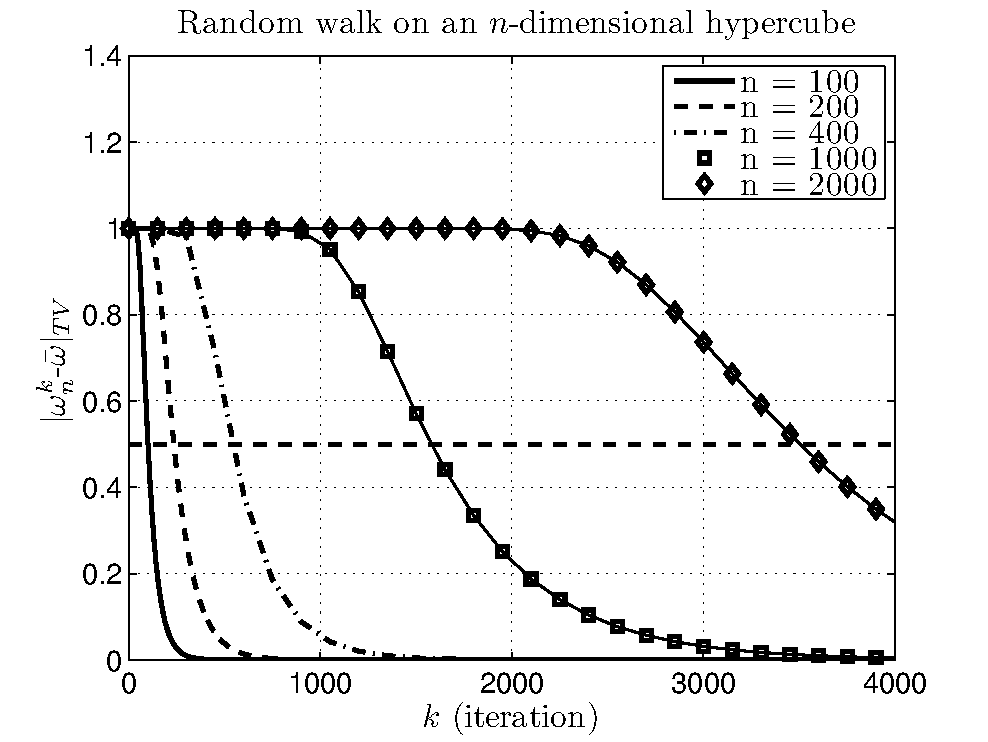
\includegraphics[width=0.7\textwidth,trim=0.6cm 0cm 0.6cm 0.8cm,clip]{rdwalk}
  }
  \caption{\label{fig:hypercube} Sample trajectories of
    $|\omega_n^k-\bar{\omega}|_{TV}$ versus iteration number $k$ for
    the random walk on a $n$-dimensional hypercube described in
    Example~\ref{ex:hypbercube}.  As $n$ increases, the trajectory
    stays close to $1$ for more iterations before it drops to zero.}
\end{figure}

Proving that a given system exhibits cutoff is typically challenging,
and only a small number of such proofs are known. In the case of the
random walk on a hypercube, an elegant method of proof uses symmetry
reduction to the so-called Ehrenfest urn problem, which has only $n +
1$ states~\cite{Diaconis1990}. In this case, the invariant
distributions $\bar{\omega}_n$ are binomial with certain means, so the
distributions $\omega^k_n$ have a shape that limits to a binomial, and
a mean that limits to the mean of $\bar{\omega}_n$. Cutoff phenomena
involve the interaction of these two processes~\cite{Lloyd2005}. For
large $n$, binomial distributions are well approximated by normal
distributions, giving the behavior~(\ref{rdwalkshape}).

\todo{MW: I compressed the long discussion that was here. Please check
  that it's still correct. \\ \\ 
  TC: OK!
  }

\todo{MW: The citation \cite{Lloyd2005} has key Lloyd2005, but none of
  the authors are Lloyd? Is this correct? \\ 
  TC: That's the first name. See \url{http://press.princeton.edu/chapters/i8113.pdf}
  }

%Although the study of cutoffs is focused on finite Markov Chains, we
%care more about what kind of linear systems can generate convergence
%trajectories that have sharp changes. It is very hard to image how a
%distribution would evolve abruptly to almost uniform from highly
%concentrated (in a single state for finite Markov Chains). However,
%there is an excellent explanation of why this happens. Consider
%another famous cutoff example: the Ehrenfest urn problem, involving
%$2$ urns and $n$ balls. In the beginning all the balls are in urn one,
%and at each iteration one of the balls is chosen randomly and put in
%the other urn. This process is a Markov Chain and it can be shown that
%this problem has the same total variation distance
%$|\omega^k_n-\bar{\omega}|_{TV}$ as the random walk on hypercubes
%problem. In fact, this is how people analyze the random walk problem
%without actually studying the $2^n$ system states. In this new Markov
%Chain, there are only $n+1$ states, which stand for the number of
%balls in urn $2$. In the beginning, all the balls are in urn $1$ so
%the probability distribution is concentrated in the first state. The
%invariant distribution of this reduced system is a binomial
%distribution centered at state $(n+1)/2$ (assuming $n$ is odd). By
%observing how the distribution is evolved when the system iterates,
%one would see two things: first, the shape of the distribution
%gradually becomes binomial to fit the final shape; secondly, the
%center of the distribution moves from $0$ toward $(n+1)/2$ at a
%certain speed (not a constant). When $n$ is large, not only does the
%center of the distribution need more iterations to move to $(n+1)/2$,
%but also the shape of the distribution needs more iterations to fit
%the stationary distribution. Cutoff is created by the combination of
%these two effects. More details about this explanation can be found in
%\cite{Lloyd2005}. Now what decides the shape of the cutoff when $n$
%tends to infinity? When $n \to \infty$, a binomial distribution can be
%well approximated by a normal distribution. Hence how the total
%variation distance changes near a cutoff can be calculated by the TV
%of two normal distributions, and it has the form like
%(\ref{rdwalkshape}). Therefore by forming the reduced system, we see
%clearly how a cutoff can happen.

\subsection{Mixing by chaotic maps}
To extend the study of cutoff phenomena to the chaotic map setting, we
begin by recalling how the Perron-Frobenius operator evolves
probability distributions for a map.

We take a space $\Omega$ with a map $S: \Omega \to \Omega$, and
we let $\Gamma$ be the set of $\omega \in L^1\Omega)$ that are
probability distributions on $\Omega$. That is, $\omega \in \Gamma$ is
non-negative and has a 1-norm of one.

\todo{MW: I introduced $\Gamma$ here for later use. I also use
  $\Omega$ directly again, rather than using $X$ for the space on
  which $S$ acts. This allows us to use $X$ later for a random
  variable.}

\todo{MW: I renamed the Perron-Frobenius operator $P_S$ just plain
  $P$. Later we have other maps (like $\phi$ and $\psi$) that also
  depend on $S$, but we don't write this on them anywhere. It looks
  strange to say that $P_S$ is related to $\psi$, when $P_S$ clearly
  depends on $S$ but $\psi$ doesn't. We could also make $\psi$ look
  like $\psi_S$, but I went with just removing $S$ everywhere. What do
  you think? \\ \\ 
  TC: Right. This looks better
  }
 
\begin{definition}
  Consider a measure space $(\Omega,\mathcal{A},\mu)$ with a map $S : \Omega \to
  \Omega$. Let $\omega \in \Gamma$, and suppose that for every $A \in
  \mathcal{A}$ the operator $P : \Gamma \to \Gamma$ satisfies
  \begin{align}
    \int_A (P \omega)(x)\mu(dx) = \int_{S^{-1}(A)} \omega(x)\mu(dx).
  \end{align}
  Then $P$ is the \emph{Perron-Frobenius operator} associated to $S$.
\end{definition}
The Perron-Frobenius operator can be thought of as evolving
probability distributions by $S$.

%%%%%%%%%%%%%%%%%%%%%%%%%%%%%%%%%%%%%%%%%%%%%%
\begin{example}[Tent map cutoff.]
  \label{ex:tentmap}
  Consider the tent map on $\Omega = [0,1]$ defined by
  \begin{align}
    \label{tentmap}
    S_\text{tent}(x) = 1-2\left|x-\frac{1}{2}\right|
  \end{align}
  with the initial distributions in $\Gamma$ given by
  \begin{align}
    \label{tentmapinitial}
    \omega_n^0 = \begin{cases}
      \frac{1}{\mu_n} &\text{ if } x \le \mu_n,\\
      0               &\text{ otherwise},
    \end{cases}
  \end{align}
  where $\mu_1 = 1$, and $\mu_{n+1} = \mu_n/2$. The Perron-Frobenius
  operator of the tent map can be explicitly computed to give
  \begin{align}
    \label{tentmapevolve}
    \omega_n^{k+1}(x) = (P_\text{tent} \omega_n^{k})(x)
    = \frac{1}{2}\left( \omega_n^{k}\left(\frac{x}{2}\right)+
      \omega_n^{k}\left(1-\frac{x}{2}\right)  \right).
  \end{align}
  The invariant distribution $\bar{\omega}$ of the tent map is
  uniform. Let $\nu_n^k = |\omega_n^k-\bar{\omega} |_{TV}$; we find
  that
  \begin{align}
    \nu_n^k =  \begin{cases}
      1- 2^{1+k-n}  &\text{ if }k \le n-1, \\
      0             &\text{ otherwise}.
    \end{cases}
  \end{align}
  The trajectories of $\nu_n^k$ with varying $n$ are shown in Figure
  \ref{tentmapcutoffplot}. It shows a cutoff.
\end{example}
\todo{TC: We use $\nu$ for a probability measure in the total variation distance definition, but we use it as a scalar in the example. Maybe we should just use $|\omega^k_n-\bar{\omega}|_{TV}$ in this example and the figure to avoid confusion?}


\begin{figure}
  \centerline{{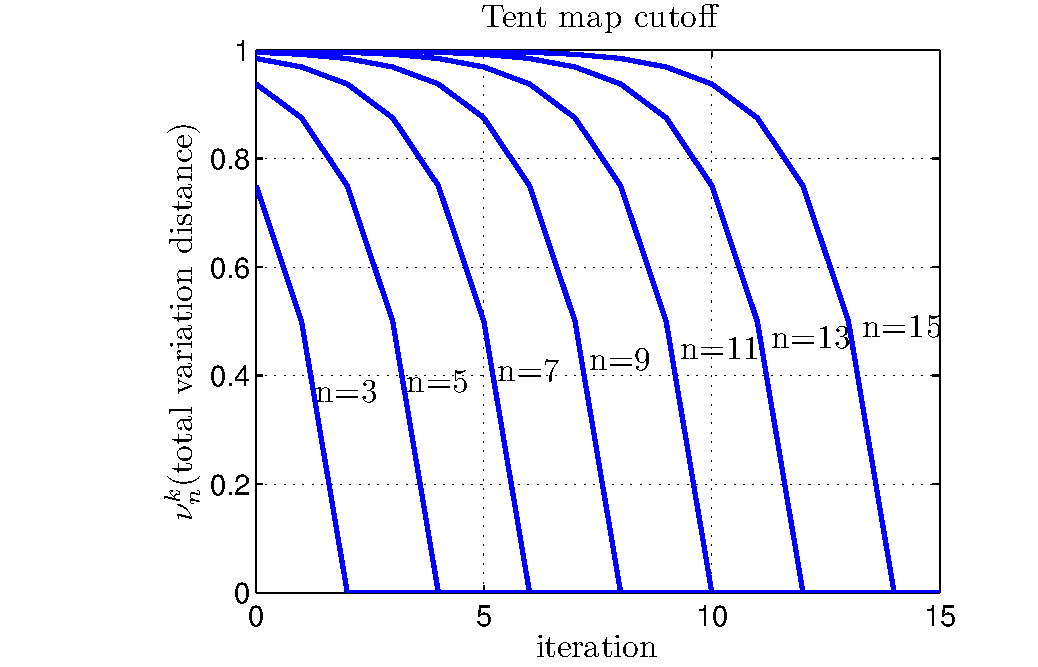
\includegraphics[width=0.8\textwidth]{tentmapcutoff}}}
  \caption{\label{tentmapcutoffplot} Trajectories of $\nu_n^k$ versus
    iteration number $k$ for the tent map described in
    Example~\ref{ex:tentmap}. This system presents a cutoff.}
\end{figure}

Hence we state the following simple theorem (a more general version is
proved in Section~\ref{sec:mainresults}).

\begin{theorem}[Tent map cutoff]
  \label{tentmapcutoff}
  The family $(\Omega,\bar{\omega},
  (\omega^k_n)_{k=0}^{\infty})_{n=1}^{\infty}$, where $\Omega =
  [0,1]$, $\bar{\omega}$ is uniform in $[0,1]$ and $\omega^k_n$ are
  defined by~(\ref{tentmapinitial}) and~(\ref{tentmapevolve}),
  presents a total variation-cutoff.
\end{theorem}
\begin{proof}
  This is a special case of Theorem~\ref{thm:mainresult1} with $m =
  1$.
\end{proof}

This example above shows that the tent map can present sharp changes
in total variation distance. We will generalize this observation to a
set of initial distributions and all 1D chaotic maps that have full
shift symbolic dynamics.

%%%%%%%%%%%%%%%%%%%%%%%%%%%%%%%%%%%%%%%%%%%%%%%%%%%%%%%%%%
%%%%%%%%%%%%%%%%%%%%%%%%%%%%%%%%%%%%%%%%%%%%%%%%%%%%%%%%%%
\section{Symbolic Dynamics and Stochastic Symbol Sequence}
\label{sec:symdyn}
%%%%%%%%%%%%%%%%%%%%%%%%%%%%%%%%%%%%%%%%%%%%%%%%%%%%%%%%%%
%%%%%%%%%%%%%%%%%%%%%%%%%%%%%%%%%%%%%%%%%%%%%%%%%%%%%%%%%%

%%%%%%%%%%%%%%%%%%%%%%%%%%%%%%
\subsection{Symbolic Dynamics}
%%%%%%%%%%%%%%%%%%%%%%%%%%%%%%

We briefly recall the definition of symbolic dynamics for chaotic
maps. We focus on 1D chaotic maps, whose symbolic dynamics are
semi-infinite sequences.

\todo{MW: I removed the notation $\mathcal{S}$ for the set of symbols,
  as we weren't really using it anywhere. \\ \\ 
  TC: OK. 
  }

Let $\{L, R\}$ be a set of emph{symbols} and define $\Sigma$ to be the
collection of all semi-infinite sequences of symbols. That is, $s\in
\Sigma$ implies
\begin{align}
  s= \{.s_0s_1\cdots s_n\cdots\}
\end{align}
with $s_i\in \{L, R\}$ for all $i$. We refer to $\Sigma$ as the
space of semi-infinite sequences of two symbols. We consider a map
$\sigma:\Sigma \to \Sigma$, called the shift map, defined by
$\sigma(s)_i = s_{i+1}$. For $s= \{.s_0s_1\cdots s_n\cdots\}$,
\begin{align}
  \sigma(s)= \{.s_1s_2\cdots s_n\cdots\}.
\end{align}
That is, the shift operator $\sigma$ simply deletes the first element
of the sequence. There are rich results about the relationship between
symbolic dynamics and chaotic maps~\cite{Wiggins1990,
  Holmes1983}. Given a map $S$ with invariant set $\Lambda$, we
partition $\Lambda = \Lambda_L \cup \Lambda_R$ into a disjoint
union. Then we define the function $\phi(x): \Lambda \to \Sigma$,
which maps a point in $x\in \Lambda$ to a semi-infinite sequence, by
\begin{align}
  \phi(x)_i = \begin{cases} L & \text{if } S^i(x) \in \Lambda_L \\
     R & \text{if } S^i(x) \in \Lambda_R. \end{cases}
\end{align}
With this definition we see that
\begin{align}
  \sigma \circ \phi = \phi \circ S.
\end{align}
Then, roughly speaking, we establish that $\phi$ is a homeomorphism,
so $S$ acting on $\Lambda$ and $\sigma$ acting on $\Sigma$ are
topologically conjugate. This relationship can be used to precisely
define the sensitivity to initial conditions of chaotic maps.

\todo{MW: I added the explicit definition of $\phi$ above. Please
  check.\\ 
  TC: Done.
  }

\todo{MW: Can we just say at the start that $\Omega$ is assumed to be
  invariant for $S$, and if it isn't we restrict $\Omega$ to be
  invariant, and then use $\Omega$ rather than introducing a new set
  $\Lambda$? \\ \\
  TC: I think this is OK. 
  }

\todo{MW: Where do we need to introduce the definition and use of
  ``full shift symbolic dynamics'' or ``full symbolic dynamics''?
  Which results depend on this? \\ \\
  TC: We use it later in the definition of $\bar{\Gamma}$ (\ref{DefOmegabar}) and lemma $3.3$, $3.4$. I am also not sure here. There is no problem to define symbolic dynamics for any maps, not just chaotic maps. So it seems the key to say this map is chaotic is the invertibility of $\phi$. Is this correct? If this is true, I believe $\psi$ is also invertible in $\Gamma$ for chaotic maps, i.e. $\bar{\Gamma} = \Gamma$. How do you think?
  }

All the results we derive in the next section for semi-infinite
stochastic symbol sequences can be extended to bi-infinite sequences
without difficulty.

%Let $\mathcal{S}=\{L, R\}$ be the set of symbols consisting of $L$ and $R$. Let $\Sigma$ be the collection of all bi-infinite sequence of elements of $\mathcal{S}$, i.e., $s\in \Sigma$ implies
% \begin{align}
% s= \{\cdots s_{-n}\cdots s_{-1}.s_0s_1\cdots s_n\cdots\}
% \end{align}
%with $s_i\in \mathcal{S}$ for all $i$. We will refer to $\Sigma$ as the space of bi-infinite sequence of two symbols. We consider a map $\sigma:\Sigma \to \Sigma$, which we shall call the shift map, defined as follows: for $s= \{\cdots s_{-n}\cdots s_{-1}.s_0\cdots s_n\cdots\}$,
%  \begin{align}
% \sigma(s)= \{\cdots s_{-n}\cdots s_{-1}s_0.s_1\cdots s_n\cdots\}
% \end{align}
%$\sigma(\cdot)$ simply shift the dot one digit to the right of the sequence. There are rich results
%about the relation between symbolic dynamics and chaotic maps. Refer to \cite{Wiggins1990, Holmes1983} for good
%references. Roughly speaking, one can say that given a chaotic map $S$, on its invariant set
%$\Lambda$, the function $\phi(x): \Lambda \to \Sigma$, which maps a point in $x\in \Lambda$
%to a bi-infinite sequence, is homeomorphism: $S$ acting on $\Lambda$ and $\sigma$ acting on
%$\Sigma$ are topologically conjugate. In other words, we have the following relation,
% \begin{align}
% S = \phi^{-1}\circ \sigma \circ \phi
% \end{align}
%And this explains the ``sensitive to initial condition'' property of chaotic maps.

%In this paper we focus on the study of $1$-D chaotic maps, whose symbolic dynamics are semi-infinite sequences in stead of bi-infinite ones. 

%Define $\hat{\Sigma}$ the collection of all
%semi-infinite sequence of elements of $\mathcal{S}$. Each of the point $x \in \Lambda$ has $s\in
%\hat{\Sigma}$ with the following form,
% \begin{align}
% s= \{.s_0s_1\cdots s_n\cdots\}
% \end{align}
%The shift operator $\sigma$ simply deletes the first element of the sequence,
% \begin{align}
% \sigma(s)= \{.s_1s_2\cdots s_n\cdots\}
% \end{align}

%%%%%%%%%%%%%%%%%%%%%%%%%%%%%%%%%%%%%%%
\subsection{Stochastic Symbol Sequences}
%%%%%%%%%%%%%%%%%%%%%%%%%%%%%%%%%%%%%%%

Since our goal is to study how the probability density is evolved by a
map, and symbolic dynamics itself does not provide this information,
we need a new object which we call a stochastic symbol sequence.

\todo{MW: I reworked this section. We only define things for $L$, not
  $\star \in \{L,R\}$, which I found too confusing. Please check that
  it's still correct.}

\begin{definition}
  A \emph{stochastic symbol sequence} $\delta$ is a semi-infinite sequence
  \begin{align}
    \delta = \{.\delta_0 \delta_1 \cdots \delta_n \cdots\},
  \end{align}
  where $\delta_i \in [0,1]$ for each $i \ge 0$. We denote the set of
  all such sequences by $\Delta$.
\end{definition}

For the symbol $L$ we define the map $\psi^L : \Gamma \to
\Delta$, which maps a probability distribution $\omega$ on $\Lambda$
to a stochastic symbol sequence $\delta^L = \psi^L(\omega)$ defined by
\begin{align}
 \label{psidef}
    \delta^L_i = \int_{\Lambda_L} (P^i \omega)(z)\,dz \text{, for all $i$,}
\end{align}
where $P$ is the Perron-Frobenius operator of map $S$. That is, if $X
\in \Lambda$ is a random variable with probability distribution
$\omega$, then
\begin{align}
  \label{deltaistar}
  \delta_i^L = \prob(\phi(X)_i = L) = \prob(S^i(X) \in \Lambda_L).
\end{align}
We see that the stochastic symbol sequence $\delta^L$ gives the
probabilities of a random point $X$ having $S^i(X)$ in $\Lambda_L$,
whereas the regular symbol sequence $s = \phi(x)$ tells us directly
whether a fixed point $x$ has $S^i(x)$ in $\Lambda_L$.

\todo{MW: I'm using the notation $X$ to indicate a random point
  variable, and $x$ to indicate non-random points. \\ \\
  TC: Looks good. 
  }

We can also define $\psi^R$ and $\delta^R$ similarly for the symbol
$R$, giving $\delta^R_i = 1 - \delta^L_i$. It is also straightforward
to extend these definitions to more than two symbols, but we will not
do so here. Later, we will write simply $\delta$ for $\delta^L$.

%\begin{example}[Symbolic representation of the tent map]
%  Let $\Lambda=[0, 1]$. Partition $\Lambda \cap
%  S^{-1}_{\text{tent}}(\Lambda)$ by writing its two components as
%  $\Lambda_L$ and $\Lambda_R$. For the tent map, $\Lambda_L=[0, 1/2]$
%  and $\Lambda_R=(1/2,1]$, we choose $\Lambda_R$ to exclude the point
%  $1/2$ to avoid the overlap. We can associate with each $x \in
%  \Lambda $ a sequence $s = \{s_i \}_{i=0}^{\infty}$ of $L$'s and
%  $R$'s defined by $s_i=j$ if $S_{\text{tent}}^i(x) \in
%  \Lambda_j$. The sequence ${s_i}$ labels the iterates of $x$
%  according to the left-right pattern they follow. In this way, we can
%  label each $x \in \Lambda$ uniquely by a semi-infinite sequence
%  $\phi(x)=s$ where the $s_i$'s are $L$'s and $R$'s. Let $\Sigma$
%  denote the space of semi-infinite sequences of two symbols $L$'s and
%  $R$'s. Then $\phi(x): \Lambda \to \Sigma$ maps a point in $x\in I$
%  to a semi-infinite sequence.  The shift operator $\sigma$ acts on
%  $s$ by simply dropping the first entry of $s$, i.e.,
%  $\sigma(\{s_i\}_{i=0}^{\infty})=\{s_i\}_{i=1}^{\infty}$. Similarly
%  the map $\psi: \bar{\Omega} \to \Delta$, where $\Delta$ denotes the
%  space of semi-infinite stochastic symbol sequence, maps an $\omega
%  \in \bar{\Omega}$ to semi-infinite stochastic symbol sequences $\{
%  \delta^L,\delta^R\}$

%Note this is different from how it acts on a bi-infinity sequence, and this demonstrates that the
%tent map ``forgets'' the past information.
%An alternative interpretation of the semi-infinite
%sequence is as follows: one can embed the 1-D map into a 2-D volume preserved map, and make the
%symbol sequence bi-infinite. However, all the $s_i$'s with $i<0$ are unobservable. We can only
%evaluate (and we only care about) the thing happened in the first dimension.
%\end{example}

\todo{MW: I removed the tent map symbol sequence example, because it
  was just repeating what had already been said. \\ \\
  TC: OK.
  }

It is clear that the map $\psi^L: \Gamma \to \Delta$, as
defined in~(\ref{psidef}), maps a probability distribution $\omega \in
\Gamma$ to the stochastic symbol sequence $\delta^L$
uniquely. Moreover, we apply the shift $\sigma$ to the stochastic
symbol sequence space $\Delta$, so that
\begin{align}
  \label{eqn:sigma_on_Delta}
  \sigma(\delta^L)_i = \delta^L_{i+1}.
\end{align}
and we see that shifts on stochastic symbol sequences
correspond to evolution by the Perron-Frobenius operator as follows.

\todo{MW: We were using $\Omega$ for the space of probability
  distributions, but this conflicts with the usage in
  Section~\ref{sec:background}, so I changed to $\Gamma$ for
  probability distributions. Is this ok? \\ \\
  TC: OK. 
  }

%%%%%%%%%%%%%%%%%%%%%%%%%%%%%%%%%%%%%%%%%%%%%%%%%%%%%%%%%%%%%
%lemma
\begin{lemma}
  The Perron-Frobenius operator $P$ on the space $\Gamma$ of
  probability distributions is related to the shift map $\sigma$ on
  the space $\Delta$ of stochastic symbol sequences by
  \begin{align}
    \psi^L \circ P = \sigma \circ \psi^L,
  \end{align}
  where $\psi^L$ is defined by~(\ref{psidef}).
\end{lemma}
\begin{proof} By definition, $\displaystyle \delta_{i+1}^L (\omega) =
  \int_{\Lambda_L} (P^{i+1} \omega)(z)dz = \int_{\Lambda_L} (P^i
  (P\omega))(z) dz = \delta_{i}^L (P \omega)$.
\end{proof}
%%%%%%%%%%%%%%%%%%%%%%%%%%%%%%%%%%%%%%%%%%%%%%%%%%%%%%%%%%%%%

However, unlike the map $\phi$ from points to (non-stochastic) symbol
sequences, the function $\psi$ mapping probability distributions to
stochastic symbol sequences is not invertible. There are many
$\omega$s that map to the same $\delta^L$. To resolve this problem,
we define a subset $\bar{\Gamma} \subset \Gamma$:
\begin{align}
  \label{DefOmegabar}
  \bar{\Gamma} = \bigg\{ \omega \in \Gamma \ \bigg|\ \omega(x) =
  \lim_{n \to \infty} \prod_{i=0}^n \beta^{\phi(x)_i}_i \text{ for
    some } \beta^L \in \Delta \text{ and } \beta^R_i = 1 -
  \beta^L_i \text{ for all } i \bigg\}.
\end{align}
Recall that $\phi(x)_i$ is the $i$-th component of the symbol sequence
of $x$ associated with the map $S$, so having full shift symbolic
dynamics is a necessary condition for having $\bar{\Gamma}$.
\todo{TC: As I described in the earlier todo, my conjecture is $\bar{\Gamma} = \Gamma$ given $\phi$ is invertible. (And $\phi$ is invertible given $S$ is chaotic.) Do you think we should try to prove it? This will not affect any later results but it makes stochastic symbol sequence much stronger.    
}

%%%%%%%%%%%%%%%%%%%%%%%%%%%%%%%%%%%%%%%%%%%%%%%%%%%%%%%%%%%%%
The following lemma justifies the existence of $\psi^{-1}$ acting on
$\bar{\Gamma}$.
%lemma
\begin{lemma} For $\omega \in \bar{\Gamma}$ corresponding to $\beta^L
  \in \Delta$ and $\delta^L = \psi^L(\omega)$, we have
 \begin{align}
    \delta^L = \beta^L.
 \end{align}
\end{lemma}
\begin{proof} By definition, $\delta_{k}^L = \int_{\Lambda_L}
  P^{k} \omega(x)dx = \int_{S^{-k}(\Lambda_L)} \omega(x)dx$, so
  from~(\ref{DefOmegabar}) we have
  \begin{align*}
    \delta_{k}^L = \lim_{n \to \infty} \sum_{\substack{s\in
        \Sigma\\s^k= L }} \prod_{i=0}^{n} \beta^{s_i}_i = \beta_k^L
    \lim_{n \to \infty} \sum_{s\in \Sigma} \prod_{\substack{i=0\\
        i\neq k}}^{n} \beta^{s_i}_i = \beta_k^L.
%    \tag*{\qedhere}
  \end{align*}
\end{proof}
%%%%%%%%%%%%%%%%%%%%%%%%%%%%%%%%%%%%%%%%%%%%%%%%%%%%%%%%%%%%%

Hence, the map $\psi^L : \Gamma \to \Delta$ is invertible on the
subset $\bar{\Gamma} \subset \Gamma$. From now on, we restrict our
attention to the space of probability distributions $\bar{\Gamma}$. It
is also easy to check that
 \begin{align}
 \label{Pconserve}
  P \omega \in \bar{\Gamma} \text{ if } \omega \in \bar{\Gamma},
 \end{align}
and since $\psi^L$ restricted to $\bar{\Gamma}$ is invertible we have
\begin{align}
  P = (\psi^L)^{-1}\circ \sigma \circ \psi^L.
\end{align}
just like (non-stochastic) symbolic dynamics. This means that the
Perron-Frobenius operator $P$ and the shift operator $\sigma$ are
conjugate in the spaces $\{\bar{\Gamma},\Delta \}$.

To further characterize the space $\bar{\Gamma}$, we give the
following lemma.

%%%%%%%%%%%%%%%%%%%%%%%%%%%%%%%%%%%%%%%%%%%%%%%%%%%%%%%%%%%%%
%lemma
\begin{lemma}
  \label{lemma:independency}
  For $X \in \Lambda$ a random variable with probability distribution
  $\omega \in \bar{\Gamma}$, and any symbol sequence $s \in \Sigma$,
  then for any $i,j$ with $i\neq j$, the events
  \begin{equation}
    \phi(X)_i=s_i \text{ and } \phi(X)_j=s_j
  \end{equation}
  are independent.
\end{lemma}

\todo{TC: there might be a better way to state the independence, and
  need to check is the proof strong enough. \\ \\
  MW: What is the conclusion here?}

%one has
% \begin{equation}
%    \prob(\phi(x)_i=s_i) =   \prob(\phi(x)_i=s_i \mid  \phi(x)_k=s_k, k= {0,\ldots,\infty\}, k \neq i )
% \end{equation}
%\end{lemma}

\begin{proof}
  Let $\delta^L = \psi^L(\omega)$ and $\delta^R = \psi^R(\omega)$, so
  \begin{align*}
    \prob(\phi(X)=s) = \lim_{n \to \infty} \prod_{i=0}^{n}
    \delta_i^{s_i} = \lim_{n \to \infty} \prod_{i=0}^{n}
    \prob(\phi(X)_i=s_i),
  \end{align*}
  where the second equality is from~(\ref{deltaistar}). This justifies
  the claim of independence.
\end{proof}
%%%%%%%%%%%%%%%%%%%%%%%%%%%%%%%%%%%%%%%%%%%%%%%%%%%%%%%%%%%%%

For any two stochastic symbol sequences, the convex combination
defined element-wise gives another stochastic symbol
sequence. Similarly, convex combinations of probability distributions
are also probability distributions. These are related as follows.

%%%%%%%%%%%%%%%%%%%%%%%%%%%%%%%%%%%%%%%%%%%%%%%%%%%%%%%%%%%%%
%lemma
\begin{lemma}
  For $\omega_1, \omega_2 \in \bar{\Gamma}$ and $\alpha\in[0,1]$, we have
  \begin{align}
    \label{psiislinear}
    \psi^L(\alpha\omega_1+(1-\alpha)\omega_2) =
    \alpha\psi^L(\omega_1)+(1-\alpha)\psi^L(\omega_2).
  \end{align}
\end{lemma}

\begin{proof}
  This follows immediately from the linearity of~(\ref{psidef}).
%  \begin{align}
%    \lefteqn{\alpha \delta^L_k(\omega_1) + (1-\alpha) \delta^L_k(\omega_2) } \nonumber\\
%                    &=   \alpha \int_{S^{-k}(\Lambda_L)} \omega_1(x)dx+
%                          (1-\alpha) \int_{S^{-k}(\Lambda_L)} \omega_2(x)dx \nonumber \\
%                    &=   \int_{S^{-k}(\Lambda_L)}\left( \alpha \omega_1(x) +(1-\alpha) \omega_2(x) \right) dx \nonumber \\
%                    &=   \delta^L_k( \alpha \omega_1 +(1-\alpha) \omega_2).
%  \end{align}
\end{proof}
%%%%%%%%%%%%%%%%%%%%%%%%%%%%%%%%%%%%%%%%%%%%%%%%%%%%%%%%%%%%%
%This property can be extended to convex combinations of $n$
%distributions.

\todo{MW: I changed the above proof. I don't think we need to write it
  all out.}

\todo{MW: Below I changed from using $\omega^*$ to $\hat{\omega}$, and
  similarly for the rest of the paper. I found the $*$ notation
  confusing.}

To use the stochastic symbol sequences $\delta^L$ and $\delta^R$
associated to a probability distributions $\omega$ for studying
cutoff, we need to express the total variation distance directly in
terms of the stochastic symbol sequences. Given $\omega, \hat{\omega}
\in \hat{\Gamma}$ with stochastic symbol sequences $\{\delta^L,
\delta^R\}$ and $\{\hat{\delta}^L,\hat{\delta}^R \}$, respectively, we
have
\begin{align}
  \label{infiniteTV}
  |\omega-\hat{\omega}|_{TV} = \frac{1}{2} \lim_{n \to \infty}
  \sum_{s\in\Sigma} \left|
    \prod_{i=0}^n\delta_i^{s_i}-\prod_{i=0}^n\hat{\delta}_i^{s_i}
  \right|.
\end{align}
This expression is difficult to evaluate in general, so let us
consider a simpler case, when $\delta^L$ and $\hat{\delta}^L$ only
have $p$ different digits, i.e.,\ $\delta_i^L = \hat{\delta}_i^L$ when
$i\notin \theta$, and $|\theta| = p$. Let $\Sigma_p$ be the space of
all symbol sequence of length $p$ with two symbols. Then we have
\begin{align}
  \label{finiteTV}
  |\omega-\hat{\omega}|_{TV} = \frac{1}{2} \sum_{s\in\Sigma_p} \left|
    \prod_{i\in
      \theta}\delta_i^{s_i}-\prod_{i\in\theta}\hat{\delta}_i^{s_i}
  \right|.
\end{align}
Importantly, we note that the total variation distance is invariant
under any simultaneous reordering of the symbols in the sequences, so
is only a function of the elements $s_i, i\in\theta$. Furthermore,
(\ref{finiteTV}) can serve as a lower bound when the symbols for
$i\notin \theta$ are unknown.

%%%%%%%%%%%%%%%%%%%%%%%%%%%%%%%%%%%%%%%%%%%%%%%%%%%%%%%%%%
\subsection{General Results}

We now turn from general stochastic symbol sequences to cases where
one of our sequences corresponds to an invariant distribution of the
map $S$. In particular, we will consider
\begin{equation}
  \label{deltabar}
  \bar{\delta}=\left\{.\frac{1}{2}\frac{1}{2}\frac{1}{2}\cdots\right\}.
\end{equation}
This is invariant under the shift operator action, so it corresponds
to an invariant distribution $\bar{\omega} =
\psi^{-1}(\bar{\delta})$. In these and future expressions, we will
write $\delta$ for $\delta^L$ and $1 - \delta$ for
$\delta^R$. Similarly, $\psi$ is the map $\psi^L$.

\todo{TC:(\ref{deltabar}) is not the only invariant measure. Any
  constant sequence is invariant under the shift map, but we are not
  interested in them. \\ \\
  MW: Do we need to say something about this?}

The following convexity lemma is the basis of all later results.
%%%%%%%%%%%%%%%%%%%%%%%%%%%%%%%%%%%%%%%%%%%%%%%%%%%%%%%%%%%%%
%lemma
\begin{lemma} For $\delta,\hat{\delta} \in \Delta$ and $\alpha\in [0,1]$,
  we have
  \begin{align}
    \label{convexityofTV}
    |\psi^{-1}(\alpha\delta+(1-\alpha)\hat{\delta})-\bar{\omega}|_{TV} \le
    \alpha|\psi^{-1}(\delta)-\bar{\omega} |_{TV}+(1-\alpha)|\psi^{-1}(\hat{\delta})-\bar{\omega}|_{TV}.
  \end{align}
\end{lemma}
\begin{proof}
  Since $\omega \mapsto |\omega-\bar{\omega}|_{TV}$ is convex, by
  using (\ref{psiislinear}) we see that $\delta \mapsto
  |\psi^{-1}(\delta)-\bar{\omega}|_{TV} $ is also convex, giving the
  desired result.
\end{proof}
%%%%%%%%%%%%%%%%%%%%%%%%%%%%%%%%%%%%%%%%%%%%%%%%%%%%%%%%%%%%%

The above lemma means that even if we cannot directly calculation the
total variation distance between stochastic symbol sequences, we can
use the convexity to deduce useful bounds.

%%%%%%%%%%%%%%%%%%%%%%%%%%%%%%%%%%%%%%%%%%%%%%%%%%%%%%%%%%%%%
%lemma
\begin{lemma}
  \label{onedifflemma} Suppose $\delta$ and $\hat{\delta}$ are two
  stochastic symbol sequences corresponding to the probability
  distributions $\omega$ and $\hat{\omega}$, respectively. Suppose
  there exists a bijection $\gamma: i \mapsto j$ such that $\delta_i =
  \hat{\delta}_j$ for all $i\in \mathbb{Z}\setminus\{k\}$. If
  $ |\delta_{k}-\frac{1}{2}| \ge
  |\hat{\delta}_{\gamma(k)}-\frac{1}{2}|$, then
 \begin{align}
      |\omega-\bar{\omega} |_{TV} \ge |\hat{\omega}-\bar{\omega} |_{TV}.
 \end{align}
\end{lemma}
\begin{proof}
  Since $|\psi^{-1}(\delta)-\bar{\omega}|_{TV}$ is independent of the
  order of the sequence, we can assume $\delta = \hat{\delta}$ for all
  $i\in \mathbb{Z}\setminus\{k\}$. Let $\tilde{\delta} =
  \delta$ for all $i\in \mathbb{Z}\setminus\{k\}$, and
  $\tilde{\delta}_{k}=1-\delta_{k}$. Then
  $|\psi^{-1}(\delta)-\bar{\omega}|_{TV}
  =|\psi^{-1}(\tilde{\delta})-\bar{\omega}|_{TV} $. When
  $|\delta_{k}-\frac{1}{2}| \ge
  |\hat{\delta}_{k}-\frac{1}{2}|$, it is always possible to
  choose $\alpha\in[0,1]$ such that $\hat{\delta}_i = \alpha \delta_i
  +(1-\alpha) \tilde{\delta}_i $.  Applying (\ref{convexityofTV}) to
  $\delta$ and $\tilde{\delta}$ with the $\alpha$ above, we have
  \begin{align*}
    |\psi^{-1}(\hat{\delta})-\bar{\omega}|_{TV}
    &\le  \alpha|\psi^{-1}(\delta)-\bar{\omega}
    |_{TV}+(1-\alpha)|\psi^{-1}(\tilde{\delta})-\bar{\omega}|_{TV} \\
    & = |\psi^{-1}(\delta)-\bar{\omega} |_{TV}.
%    \tag*{\qedhere}
  \end{align*}
\end{proof}
%%%%%%%%%%%%%%%%%%%%%%%%%%%%%%%%%%%%%%%%%%%%%%%%%%%%%%%%%%%%%

%%%%%%%%%%%%%%%%%%%%%%%%%%%%%%%%%%%%%%%%%%%%%%%%%%%%%%%%%%%%%
%lemma
\begin{lemma}
  \label{alldifflemma} Suppose $\delta$ and $\hat{\delta}$ are two
  stochastic symbol sequences corresponding to the probability
  distributions $\omega$ and $\hat{\omega}$, respectively. Suppose
  there exists a bijection $\gamma: i \mapsto j$ such that
  $|\delta_i-\frac{1}{2}| \ge |\hat{\delta}_j-\frac{1}{2} |$ for all
  $i\in \mathbb{Z}$. Then
  \begin{align}
    |\omega-\bar{\omega} |_{TV} \ge|\hat{\omega}-\bar{\omega} |_{TV}.
  \end{align}
\end{lemma}
\begin{proof} Apply Lemma \ref{onedifflemma} repeatedly.
\end{proof}
%%%%%%%%%%%%%%%%%%%%%%%%%%%%%%%%%%%%%%%%%%%%%%%%%%%%%%%%%%%%%

The above lemma allows us to compare $|\omega-\bar{\omega}|_{TV}$ and
$|\hat{\omega}-\bar{\omega}|_{TV}$ if some relation of their
stochastic symbol sequences is known. Now for a given $\omega$ we want
to bound $|\omega-\bar{\omega}|_{TV}$ by choosing an $\hat{\omega}$
such that $|\hat{\omega}-\bar{\omega}|_{TV}$ is easy to calculate. The
choices we make are the sequences with the following form:
\begin{align}
  \begin{split}
    \label{deltamM}
    \delta^m &= \{.\underbrace{m \, m \cdots m}_{\text{$p$ times}}\frac{1}{2}\frac{1}{2}\cdots \}, \\
    \delta^M &= \{.\underbrace{M \, M \cdots M}_{\text{$p$ times}}\frac{1}{2}\frac{1}{2}\cdots \}.
  \end{split}
\end{align}
As we will see later, $|\omega-\bar{\omega}|_{TV}$ can be evaluated
easily for such sequences.

\todo{MW: We used to have a notation where the leading elements of
  these sequences were $\delta^m_{\star}$, etc, but I think the
  notation above is simpler.}
  
%Where $\delta^m_0=\delta^m_1= \cdots = \delta^m_{p-1} \equiv \delta^m_{\star}$ and
%$\delta^M_0=\delta^M_1= \cdots = \delta^M_{p-1}\equiv \delta^M_{\star}$.


%First we are going to generalize the lower bound result from $\delta_i=1$, for $i\in \theta$ to $\delta_i=\delta^M$. Note here $\delta^M$ is a number, $1/2 \le \delta^M \le 1$.

%%%%%%%%%%%%%%%%%%%%%%%%%%%%
\subsubsection{Lower Bound}
%%%%%%%%%%%%%%%%%%%%%%%%%%%%%

We now construct an explicit lower bound for the total variation,
using the framework above.

%%%%%%%%%%%%%%%%%%%%%%%%%%%%%%%%%%%%%%%%%%%%%%%%%%%%%%%%%%%%%
%theorem
\begin{theorem}
  \label{theoremlb} Suppose $\delta$ and $\bar{\delta}$ are two
  stochastic symbol sequences corresponding to the probability
  distribution $\omega$ and the invariant distribution $\bar{\omega}$,
  respectively, with $\bar{\delta}$ being~(\ref{deltabar}). Suppose
  there is a set $\theta \subset \mathbb{N}_0 = {0,1,2,\ldots}$,
  $|\theta|=p$, such that for all $i \in \theta$,
  $|\delta_i-\frac{1}{2}|>|m-\frac{1}{2}|$. Then
  \begin{align}
    \label{lbineq}
    |\omega-\bar{\omega}|_{TV} \ge
    \mathbf{I}_{\frac{1}{2}}(p-q^*,q^*+1) -
    \mathbf{I}_{1-m}(p-q^*,q^*+1),
  \end{align}
  where
  \begin{align}
    \label{kstar}
    q^* = \left\lfloor p \frac{\log{2}+\log{(\frac{1}{2}-\epsilon)}
      }{\log{(\frac{1}{2}-\epsilon)}-\log{(\frac{1}{2}+\epsilon})}
    \right\rfloor,
  \end{align}
  $\epsilon = |m-\frac{1}{2}|$, and $\mathbf{I}$ is the regularized
  incomplete beta function.
\end{theorem}
\begin{proof}
  Since the total variation is independent of the order of the sequence, we can
  assume that $\theta=\{0,1,\ldots,p-1\}$. Also, without loss of
  generality, we assume for $i\in \theta$, $\delta_i \ge
  \epsilon+\frac{1}{2}= m$. Using equation (\ref{finiteTV}) and Lemma
  \ref{alldifflemma}, we have
  \begin{align}
    \label{lbtv}
    |\omega-\bar{\omega}|_{TV} &\ge \frac{1}{2} \sum_{s\in\Sigma_p}
    \left| \prod_{i\in \theta}\delta_i^{s_i}-\prod_{i\in\theta}\bar{\delta}_i^{s_i}  \right| \nonumber\\
    &\ge \frac{1}{2} \sum_{q=0}^{p}
    {p \choose q} \left|m^q (1-m)^{p-q} - \frac{1}{2^p} \right| \nonumber \\
    &= \frac{1}{2} \sum_{q=0}^{p} \left|{p \choose q} m^q
      (1-m)^{p-q} -{p \choose q} \frac{1}{2^p} \right|.
  \end{align}

  \todo{TC: The first line is an inequality because $p < \infty$. \\ \\
    MW: Do we need to say something about this?}

  \todo{MW: The proof used to stop here, but I shifted the text below
    into the proof as well, as it seems to belong here. Is this ok?}
  
  %%%%%%%%%%%%%%%%%%%%%%%%%%%%%%%%%%%%%%%%%%%%%%%%%%%%%%%%%%%%% 
  
  So the total variation distance can be lower bounded by the
  difference between two binomial distributions. We can find their
  difference by subtracting their cumulative distribution functions at
  the point where they cross over each other. To do this, we need to find
  the point where the first distribution begins to exceed the second
  distribution. That is, to find the largest $q^*$ such that
  \begin{align}
    \left(\frac{1}{2}+\epsilon\right)^{q^*}\left(\frac{1}{2} -
      \epsilon\right)^{p-1-q^*}-2^{-p} \le 0.
  \end{align}
  Solving for $q^*$ gives~(\ref{kstar}). Now the cumulative
  distribution function of a binomial distribution can be expressed in
  terms of the regularized incomplete beta function $\mathbf{I}$ as
  follows. For the distribution $\text{binomial}(r,p)$, its cumulative
  distribution function is
  \begin{align}
    F(q;p,r) = \mathbf{I}_{1-r}(p-q,q+1).
  \end{align}
  Substituting $q^*$ into $q$, and $1/2$ and $m$ into $r$, we
  obtain~(\ref{lbineq}).
  % \begin{align}
  %   |\omega-\bar{\omega}|_{TV} \ge \mathbf{I}_{\frac{1}{2}}(p-k^*,k^*+1) - \mathbf{I}_{1-\delta^m}(p-k^*,k^*+1)
  % \end{align}
\end{proof}

An interesting corollary is that as $p$ goes to $\infty$,
$|\omega-\bar{\omega}|_{TV}$ goes to $1$ for all $\epsilon>0$. So each
of the constant stochastic symbol sequences correspond to an invariant
measure of the map.

%%%%%%%%%%%%%%%%%%%%%%%%%%%
\subsubsection{Upper Bound}
%%%%%%%%%%%%%%%%%%%%%%%%%%%

We have seen that for a constant sequence with components not equal to
$1/2$, the total variation distance to the invariant distribution
$\bar{\omega}$ is $1$ from the previous theorem. Hence this result
does not give us any information about the upper bound. We would like
to bound the distance by the sum of the sequence, and give the
following theorem.

\todo{MW: I added the specification below (and in
  Theorem~\ref{theoremlb}) that $\bar{\delta}$ is
  from~(\ref{deltabar}). Please check.}

\begin{theorem}
  \label{theoremub}Suppose $\delta$ and $\bar{\delta}$ are two
  stochastic symbol sequences corresponding to the probability
  distribution $\omega$ and the invariant distribution $\bar{\omega}$,
  respectively, with $\bar{\delta}$ being~(\ref{deltabar}). Suppose
  \begin{align}
    \sum_{i=0}^\infty \Big|\delta_i - \frac{1}{2}\Big| = \frac{M}{2}.
  \end{align}
  Then    
  \begin{align}
    |\omega-\bar{\omega}|_{TV} \le \begin{cases}
      \rho - 2^{-\lceil M \rceil } &\text{ if } \rho>1-2^{-\lceil M \rceil }\\
      1-2^{-\lfloor M \rfloor}    &\text{ otherwise},\\
    \end{cases} 
  \end{align}
  where $\rho = \frac{1}{2} +  \frac{M-\lfloor M \rfloor}{2}$.
\end{theorem}
\begin{proof}
  With the convexity inequality (\ref{convexityofTV}), one can show
  that for a set of stochastic symbol sequences
  $(\delta^j)_{j=1}^\infty$ and coefficients $(\alpha_j)_{j=1}^\infty$
  with $\alpha_j \in [0,1]$ and $\sum_{j=1}^\infty \alpha_j = 1$, we
  have
  \begin{align}
    \sum_j \alpha_j\Big|\psi^{-1}(\delta^j)-\bar{\omega}\Big|_{TV} \ge
    \bigg|\psi^{-1}\Big(\sum_j \alpha_j \delta^j\Big)-\bar{\omega}\bigg|_{TV}.
  \end{align}
  So for each $M$, if we can express $\delta$ as the convex
  combination of a set of $\delta^j$, then the total variation
  distance $|\omega-\bar{\omega}|_{TV}$ can be bounded by the total
  variation of individual $\delta^j$. Let us define the set
  $\mathbf{C} = \{\delta \in \Delta \mid \sum_i|\delta_i-\frac{1}{2}|
  = \frac{M}{2}\}$. It is easy to see that $\mathbf{C} =
  \operatorname{conv} \mathbf{D}$, the convex hull of $\mathbf{D}$,
  where $\mathbf{D}$ is defined as
  \begin{align}
    \mathbf{D}=\Big\{\delta \in \Delta \ \Big|\ \delta \text{ has } \lfloor M \rfloor
    \text{ } 1\text{'s, one } M-\lfloor M \rfloor \text{, and all
      other elements are }\frac{1}{2} \Big\},
  \end{align}
  and $|\psi^{-1}(\delta)-\bar{\omega}(x)|_{TV}$ for each $\delta \in
  \mathbf{D}$ can be calculated as
  \begin{align}
    |\psi^{-1}(\delta)-\bar{\omega}(x)|_{TV} =
    \begin{cases}
      \rho - 2^{-\lceil M \rceil } &\text{ if } \rho>1-2^{-\lceil M \rceil }\\
      1-2^{-\lfloor M \rfloor} &\text{ otherwise},
    \end{cases}
  \end{align}
  where $\rho = \frac{1}{2} + \frac{M-\lfloor M \rfloor}{2}$. We
  obtain the upper bound by choosing the set of $\delta^j$ to be
  $\mathbf{D}$.
\end{proof}

\todo{MW: We do mean the convex hull with
  $\operatorname{conv}\mathbf{D}$, correct?}

Unfortunately, the above upper bound is in general not very tight. We
state it just to inspire the next theorem, which gives a tighter
bound.
%%%%%%%%%%%%%%%%%%%%%%%%%%%%%%%%%%%%%%%%%%%%%%%%%%%%%%%%%%%%%%%%%%%%%%%%%%%%%%%%%%%%%%%%

\begin{theorem}
  \label{theoremub2}
  Suppose $\delta$ and $\bar{\delta}$ are two stochastic symbol
  sequences corresponding to the probability distribution $\omega$ and
  the invariant distribution $\bar{\omega}$, respectively, with
  $\bar{\delta}$ being~(\ref{deltabar}). Suppose
  \begin{align}
    \sum_{i=0}^\infty \Big|\delta_i - \frac{1}{2}\Big| = \frac{M}{2},
  \end{align}
  and $\delta_i \le M$ for all $i$. Then
  \begin{align}
    \label{ubineq}
    |\omega-\bar{\omega}|_{TV} \le
    \mathbf{I}_{\frac{1}{2}}(p-q^*,q^*+1) -
    \mathbf{I}_{1-M}(p-q^*,q^*+1)
  \end{align}
  with
  \begin{align}
    \label{kstarub}
    q^* = \left\lfloor p \frac{\log{2}+\log{(\frac{1}{2}-\epsilon)}
      }{\log{(\frac{1}{2}-\epsilon)}-\log{(\frac{1}{2}+\epsilon})}
    \right\rfloor,
  \end{align}
  where $\epsilon = |M - \frac{1}{2}|$ and $p = \lceil
  \frac{M}{2\epsilon}\ \rceil$.
\end{theorem}

\begin{proof}
  Similarly to the previous proof, let
  \begin{align}
    \mathbf{D}=\Big\{\delta \in \Delta \ \Big|\ \delta \text{ has }
    (p-1)\text{ } of \text{ } M\text{'s, one } M-(p-1) M \text{, and
      all other }\delta_i\text{'s are }\frac{1}{2} \Big\}.
  \end{align}
  Then the set $\mathbf{C} = \{\delta \in \Delta \mid
  \sum_i|\delta_i-\frac{1}{2}| = \frac{M}{2}\}$ is the convex hull
  $\mathbf{C} = \operatorname{conv} \mathbf{D}$. All $\delta \in
  \mathbf{D}$ have the same value of $|\psi^{-1}(\delta) -
  \bar{\omega}|_{TV} $ and this is bounded by
  \begin{align}
    \label{middleineq}
    |\psi^{-1}(\delta) - \bar{\omega}|_{TV} < |\psi^{-1}(\delta^M) -
    \bar{\omega}|_{TV},
  \end{align}
  and $|\psi^{-1}(\delta^M) - \bar{\omega}|_{TV}$ can be calculated in
  a similar fashion to that in the lower bound proof by finding the
  $q^*$ such that the first binomial distribution is less than the
  second one, i.e., find the smallest $q^*$ such that
  \begin{align}
    \left(\frac{1}{2}+\epsilon\right)^{q^*} \left(\frac{1}{2} -
      \epsilon\right)^{p-q^*}-2^{-p} \ge 0.
  \end{align}
  Once $q^*$ is solved as in~(\ref{kstarub}), we have
  $|\psi^{-1}(\delta^M) - \bar{\omega}|_{TV} =
  \mathbf{I}_{\frac{1}{2}}(p-q^*,q^*+1) -
  \mathbf{I}_{1-M}(p-q^*,q^*+1)$. Combining this
  with~(\ref{middleineq}), we obtain~(\ref{ubineq}).
\end{proof}

%%%%%%%%%%%%%%%%%%%%%%%%%%%%%%%%%%%%%%%%%
% approximated lower and upper bound
%%%%%%%%%%%%%%%%%%%%%%%%%%%%%%%%%%%%%%%%%
The above lower and upper bound theorems can be applied to any given
stochastic symbol sequence so long as one can find $\delta^m$ and
$\delta^M$ to bound it. In the following theorem, we consider a
scenario in which $p \to \infty$ and $m \to 1/2$ (or $M \to 1/2$), and
we calculate where the lower and upper bounds converge to.

%%%%%%%%%%%%%%%%%%%%%%%%%%%%%%%%%%%%%%%%%%%%%%%%%%%%%%%%%
\begin{theorem}
  \label{theoremapproxlb} Suppose $\bar{\omega}$ and
  $\omega_{\text{lb}}$ (resp.\ $\omega_{\text{ub}}$) are two
  probability distributions with stochastic symbol sequences
  $\bar{\delta}$ and $\delta^m$ (resp.\ $\delta^M$) as defined in
  (\ref{deltabar}) and (\ref{deltamM}), respectively. If $p \to
  \infty$ and $m \to \frac{1}{2}$ (resp.\
  $M \to 1/2$), then we have
  \begin{align}
    \begin{split}
      \label{lbublimit}
      |\omega_{\text{lb}}-\bar{\omega}|_{TV}
      & =  \erf \left( \sqrt{\frac{p}{2}}\left(m-\frac{1}{2}\right)\right), \\
      \text{resp. }  |\omega_{\text{ub}}-\bar{\omega}|_{TV}
      & =  \erf \left( \sqrt{\frac{p}{2}}\left(M-\frac{1}{2}\right)\right).
    \end{split}
  \end{align}
\end{theorem}
\begin{proof}
  When $p\to \infty$, the binomial distribution approaches the normal
  distribution as $\operatorname{Binom}(m,p) \to \mathcal{N}(pm,
  pm(1-m))$.  The term $|\omega_{\text{lb}}-\bar{\omega}|_{TV}$ thus
  equals the total variation between two normal distributions, which
  can be evaluated by subtracting their cumulative distribution
  functions:
  \begin{align}
    |\omega_{\text{lb}}-\bar{\omega}|_{TV} &=
    \frac{1}{2}\left(1+\erf\left(\frac{x^*-pm}{\sqrt{2pm(1-m)}}\right)\right)
    -\frac{1}{2}\left(1+\erf\left(\frac{x^*-p\frac{1}{2}}{\sqrt{2p\frac{1}{2}(1-\frac{1}{2})}}\right)\right) \nonumber\\
    &=\erf\left(\frac{x^*-pm}{\sqrt{2pm(1-m)}}\right)-
    \erf\left(\frac{x^*-p\frac{1}{2}}{\sqrt{2p\frac{1}{2}(1-\frac{1}{2})}}\right),
  \end{align}
  where $x^*$ is the point at which the two distributions cross. When
  $m \to \frac{1}{2}$, the denominators in both $\erf(\cdot)$ are the
  same, and hence the variances of the two normal distributions are
  the same while the means differ by $p(m-\frac{1}{2})$, and we
  obtain~(\ref{lbublimit}). The same argument holds for the
  $\omega_{\text{ub}}$ equality.
\end{proof}




%Just like the lower bound, we can also give an approximate upper bound,
%\begin{theorem}
%\label{theoremapproxub}  $\delta$ and $\bar{\delta}$ are two stochastic symbol sequences, each
%corresponds to the probability distribution $\omega$ and the invariant distribution $\bar{\omega}$,
%respectively. Suppose $\sum_{i=0}^\infty |\delta_i - \frac{1}{2}| = \frac{M}{2}$, and $p$ is large
%and $\delta^M_\star$ close to $\frac{1}{2}$, then
%\begin{align}
%\label{lbineqapprox}
%    |\omega-\bar{\omega}|_{TV}   \le  \erf\left( \sqrt{p}\left(M-\frac{1}{2}\right)\right)
%\end{align}


%\end{theorem}
%\paragraph{proof} Similar to theorem \ref{theoremapproxlb}




%%%%%%%%%%%%%%%%%%%%%%%%%%%%%%%%%%%%%%%%%%%%%%%%%%%%%%%%%%
%%%%%%%%%%%%%%%%%%%%%%%%%%%%%%%%%%%%%%%%%%%%%%%%%%%%%%%%%%
\section{Main results}
\label{sec:mainresults}
%%%%%%%%%%%%%%%%%%%%%%%%%%%%%%%%%%%%%%%%%%%%%%%%%%%%%%%%%%
%%%%%%%%%%%%%%%%%%%%%%%%%%%%%%%%%%%%%%%%%%%%%%%%%%%%%%%%%%

In the previous section we only dealt with the relation between fixed
$\omega$ and $\bar{\omega}$, with no evolution. In this section use
our results to bound $|\omega^k-\bar{\omega}|_{TV}$ when $\omega^k$ is
evolved by the Perron-Frobenius operator $\omega^{k+1} = P \omega^k$
and so the corresponding stochastic symbol sequence $\delta^k$ evolves
with the shift map $\sigma$.

We begin by considering two examples, where given stochastic symbol
sequences, we can observe how the corresponding values of
$|\omega^k-\bar{\omega}|_{TV}$ change.

\begin{example}
  \label{example:constantoega0}
  Suppose the initial probability distribution $\omega^0$ has the
  stochastic symbol sequence
  \begin{align}
    \label{constantomega0}
    \psi(\omega^0) = \Big\{.\underbrace{m \, m \cdots m}_{\text{$p$
        times}}\frac{1}{2}\frac{1}{2}\cdots\Big\},
  \end{align}
  with $m >\frac{1}{2}$, and $\bar{\omega}$ corresponds
  to~(\ref{deltabar}). Now $\omega^k$ evolves so that the
  corresponding symbol sequence $\delta^k$ is shifted, with
  $\delta^{k+1} = \sigma(\delta^k)$. It is then obvious that
  $|\omega^p-\bar{\omega}|_{TV} = 0$.

  However, how sharp is the change from the initial distance to zero?
  This depends both on $p$ and $m$. We plot the trajectories of
  $|\omega^0-\bar{\omega} |_{TV}$ versus $p$ for $m=\{0.6,
  0.7,0.8,0.9\}$ in the right plot of
  Figure~\ref{deltaMexample1}. Note that one can also regard these
  figures as showing $|\omega^k-\bar{\omega}|_{TV}$ versus $k$ with
  fixed $p=300$ for $\psi(\omega^0)$, because the shift operator
  removes one $m$ in the sequence per iteration.
  
  When $m=1$, the trajectory is already shown in
  Figure~\ref{tentmapcutoffplot} for the tent map. Now from
  Figure~\ref{deltaMexample1} we see that even when $m < 1$, we still
  observe the concave sharp change before the total variation goes to
  zero.

  An easier way to see why the concave trajectories occur is to plot
  the distributions $\omega$ and $\bar{\omega}$ in a reduced space. We
  know that
  \begin{align}
    |\omega-\bar{\omega}|_{TV} &= \frac{1}{2} \sum_{s\in\Sigma_{p}}
    \left| \prod_{i=0}^p\delta_i^{s_i}-\prod_{i=0}^p\bar{\delta}_i^{s_i}  \right| \nonumber\\
    &= \frac{1}{2} \sum_{q=0}^p
    {p \choose q} \left|m^q (1-m)^{p-q} - \frac{1}{2^p} \right| \nonumber \\
    &= \frac{1}{2} \sum_{q=0}^p \left|{p \choose q} m^q (1-m)^{p-q}
      -{p \choose q} \frac{1}{2^p} \right|.
    \label{eqn:constantoega0_binomials}
  \end{align}
  Figure~\ref{deltaMexample1} (left) plots the two terms ${p \choose
    q} m^q (1-m)^{p-q}$ and ${p \choose q} \frac{1}{2^p}$ using $p/q$
  as the horizontal axis and with $m = 0.7$. We see that when $p$ is
  small there is greater overlap, causing the drop in total variation.
\end{example}

\todo{MW: I reworded the last paragraph above. Please check.}

\todo{TC: correct the x-axis in Figure \ref{deltaMexample1} from $i$
  to $p$, and what is the y-axis? \\ \\
  MW: Does this still need to be done?}

\todo{TC: In the right plot of Figure \ref{deltaMexample1}, the legend
  is $m$ not $\delta^M$. \\ \\
  MW: I guess this still needs to be done?}

\begin{figure}
  \centerline{
    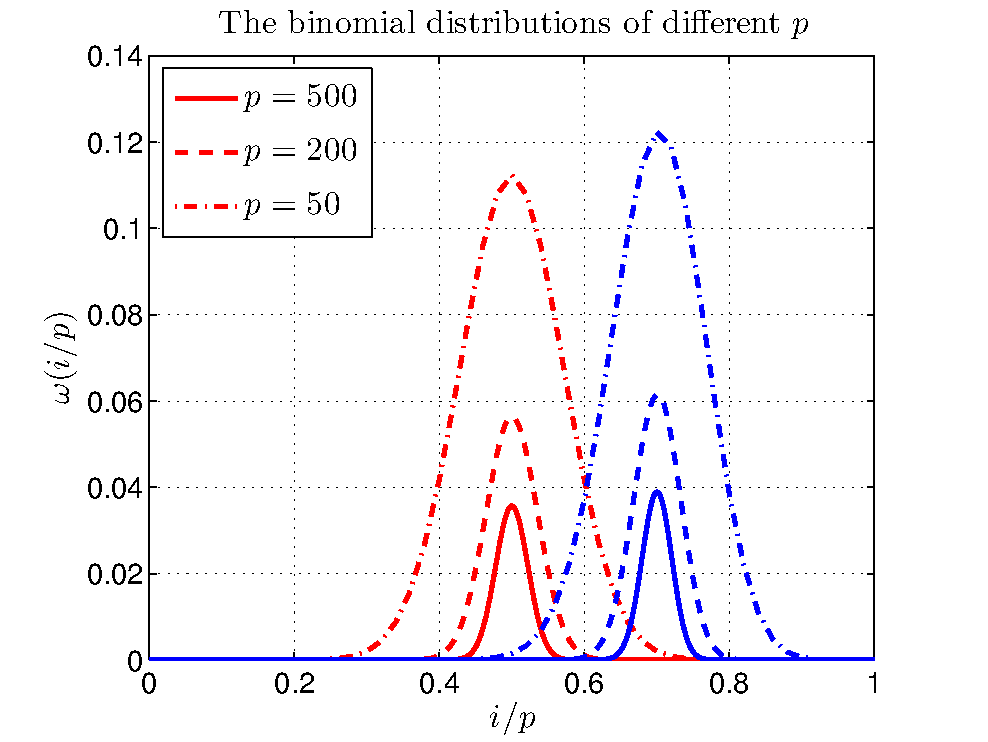
\includegraphics[width=0.5\textwidth,trim=25 0 45 0,clip]{deltaMexample1a}
    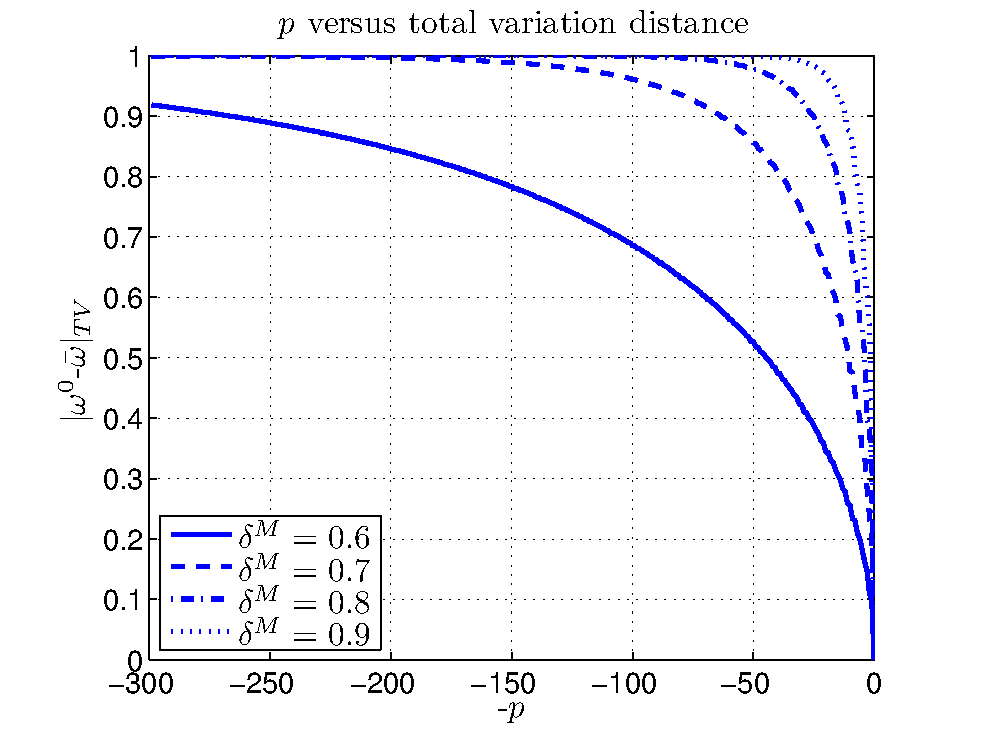
\includegraphics[width=0.5\textwidth,trim=25 0 45 0,clip]{deltaMexample1b}
  }
  \caption{\label{deltaMexample1} Left: comparison of the binomial
    distributions from~(\ref{eqn:constantoega0_binomials}). The value
    of $|\omega^0-\bar{\omega}|_{TV}$, where $\omega^0$ has the
    form~(\ref{constantomega0}), can be evaluated by finding the
    overlap area these two binomials.  When $p$ is large, the overlap
    area is smaller, so the total variation is smaller. Right: the
    variation of $|\omega^0-\bar{\omega}|_{TV}$ with $p$ for different
    values of $m$. Evolving the distribution~(\ref{constantomega0}) is
    equivalent to changing $p$, so this set of trajectories can be
    also interpreted as $|\omega^k-\bar{\omega}|_{TV}$ for $k=300-p$.}
\end{figure}

From the above example, we can give the following theorem.
\begin{theorem}
  \label{thm:mainresult1}
  For a 1D map $S:\Lambda \to \Lambda$ with full shift symbolic
  dynamics, define the family
  $(\Omega,\bar{\omega},(\omega^k_n)_{k=0}^{\infty})_{n=1}^{\infty}$
  by the initial condition $\omega^0_n\in\bar{\Gamma}$ satisfying
  \begin{equation}
    \label{eqn:mainresult1_IC}
    \psi(\omega^0_n) =  \{.\underbrace{m m \cdots m}_{n}\frac{1}{2}\frac{1}{2}\cdots\} 
  \end{equation}
  for $0 \le m \le 1$, and the evolution $\omega^{k+1} = P \omega^k$
  by the Perron-Frobenius operator $P$. Then this sequence presents a
  total variation cutoff.
\end{theorem}
\todo{MW: Theorem statement reworded, please check.}
\begin{proof}
  Let $t_n = n$. When $k_n>(1+\epsilon)n$, then
  $|\omega^k_n-\bar{\omega}|_{TV}=0$. When $k_n<(1-\epsilon)n$, then
  $n-k_n>\epsilon n$, and so
  \begin{align*}
    |\omega_n^{k_n}-\bar{\omega}|_{TV} &   = |\omega_n^{n-{(n-{k_n})}}-\bar{\omega}|_{TV} \\
    & \ge |\omega_n^{n-{\lceil\epsilon n \rceil}}-\bar{\omega}|_{TV}\\
    &   = |\omega_p^{{p-{\lceil\epsilon n \rceil}}}-\bar{\omega}|_{TV}  \text{ for any } p\ge n \\
    &\to 1 \text{ as } n \to \infty.
%    \tag*{\qedhere}
  \end{align*}
\end{proof}

Theorem \ref{tentmapcutoff} is a special case of
Theorem~\ref{thm:mainresult1} with $m = 1$.

%%%%%%%%%%%%%%%%%%%%%%%%%%%%%%%%%%%%%%%%%%%%%%%%%%%%%%%%%%%%%%%%%%%%%%%%%%%%%%%%%%
\begin{example}
  \label{ex:exp_entries}
  Suppose $\omega^0$ has the stochastic symbol sequence
  \begin{align}
    \label{expw0}
    \psi(\omega^0) =  \{.\delta_0 \delta_1 \delta_2 \cdots\},
  \end{align}
  where $\delta_i = \frac{1}{2} + \epsilon r^i$, $\epsilon \in
  [0,1/2]$ and $r\in [0,1]$. We choose it to decay geometrically so we
  can use the upper bound theorem with fixed $p$. The area under
  $\delta$ and above $\frac{1}{2}$ can be calculated by the sum of a
  geometric series, as follows. Let $M^k = \delta_k$; then
  \begin{align}
    \frac{M_k}{2} = \frac{\delta_k}{1-r}.
  \end{align}
  We thus choose $p = \lfloor \frac{1}{1-r} \rfloor$ for the upper
  bound Theorem~\ref{theoremub2}. Now $p$ is a constant, so the analysis is easier. We
  use the same $p$ for the lower bound Theorem~\ref{theoremlb}, so $m^k =
  r^p(\delta_{k}-\frac{1}{2}) $. From the upper and lower bound
  theorems, the total variation distance to the stationary
  distribution at iteration $k$ can be bounded by
  \begin{align}
    \label{omegakbound}
    |\psi^{-1}((\delta^m)^k)-\bar{\omega}|_{TV}
    <|\omega^k-\bar{\omega}|_{TV}<|\psi^{-1}((\delta^M)^k)-\bar{\omega}|_{TV},
  \end{align}
  where
  \begin{align}
    \label{defdeltamM}
    (\delta^m)^k = \{.\underbrace{m^k m^k \cdots m^k}_{\text{$p$ times}}
    \frac{1}{2}\frac{1}{2}\cdots\}, \nonumber\\
    (\delta^M)^k = \{.\underbrace{M^k M^k \cdots M^k}_{\text{$p$ times}}
    \frac{1}{2}\frac{1}{2}\cdots\}.
  \end{align}

  \todo{MW: I added references to the upper bound
    Theorem~\ref{theoremub2} and lower bound Theorem~\ref{theoremlb}
    above. Please check these are the right ones.}
  
  This is valid for each $k$. The left plot of
  Figure~\ref{deltaMexample2} shows how the upper bound distribution
  moves toward the binomial distribution centered at $p/2$ as $k$
  increases, causing the drop in total variation as they overlap. The
  right plot of Figure~\ref{deltaMexample2} shows the upper and lower
  bounds versus iteration number $k$ for $\delta_0= 1$ and $r=0.998$.
  We see the concave shape caused by the comparatively rapid
  overlapping of the distributions in the left plot.
  
  We stress that finding the actual $|\omega^k-\bar{\omega}|_{TV}$
  trajectory is infeasible because we would need to
  evaluate~(\ref{infiniteTV}) for each $\omega^k$. Even just to find
  an approximation using~(\ref{finiteTV}) is very expensive. This
  demonstrates the value of the upper and lower bound theorems. Even
  so, we do not get much insight on how the bounds evolve because
  these two theorems give bounds based on the incomplete beta
  function. Based on Theorem~\ref{theoremapproxlb}, we see that even
  when we do not have $p \to \infty$ and $m \to 1$, we still have the
  approximate bounds
  \begin{align}
    \label{expub}
    |\omega^k -\bar{\omega}|_{TV}
    &\lesssim
    \erf\left( \sqrt{\frac{p}{2}}\left(M^k
        - \frac{1}{2}\right)\right)
    = \erf\left( \sqrt{\frac{1}{2(1-r)}}
      \epsilon^0r^k \right) \\
    \label{explb}
    |\omega^k -\bar{\omega}|_{TV} &\gtrsim \erf\left(
      \sqrt{\frac{1}{2(1-r)}} \epsilon^0 r^{\frac{1}{1-r}}r^k \right)
    = \erf\left( \sqrt{\frac{1}{2(1-r)}} \epsilon^0 e^{-1} r^k
    \right).
  \end{align}
  These approximate upper and lower bounds are also plotted on the
  right of Figure~\ref{deltaMexample2}, and we see that they are
  almost identical to the true bounds.

  Both~(\ref{explb}) and~(\ref{expub}) show the normal shape, just
  like we saw in Example~\ref{ex:hypbercube}. Since $M^k-\frac{1}{2} =
  \epsilon^0 r^k$ decays exponentially (with factor $r$) to $0$, the
  trajectory does not look like the error function itself. Instead, it
  has a sharper change before the cutoff occurs and decays more mildly
  after it.
\end{example}
%%%%%%%%%%%%%%%%%%%%%%%%%%%%%%%%%%%%%%%%%%%%%%%%%%%%%%%%%%%%%%%%%%%%%%%%%%%%%%%%%%%%

\todo{MW: I changed~(\ref{explb}) and~(\ref{expub}) to use $\lesssim$
  and $\gtrsim$ symbols. Is this clear?}

\begin{figure}
  \centerline{
    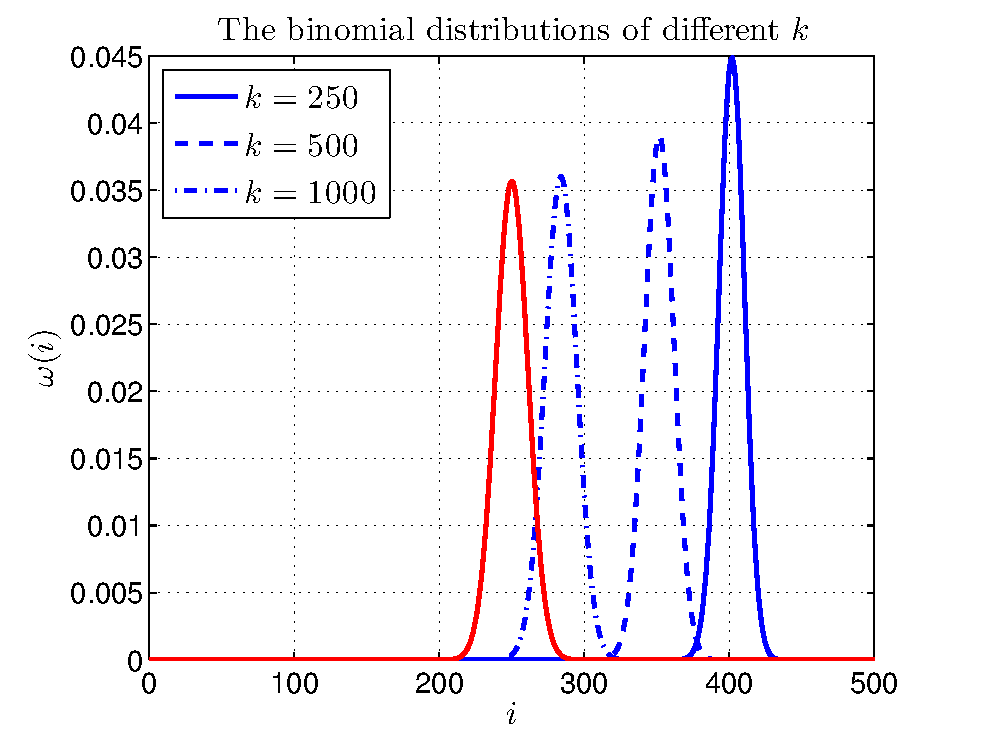
\includegraphics[width=0.5\textwidth,trim=15 0 42 0,clip]{deltaMexample2a}
    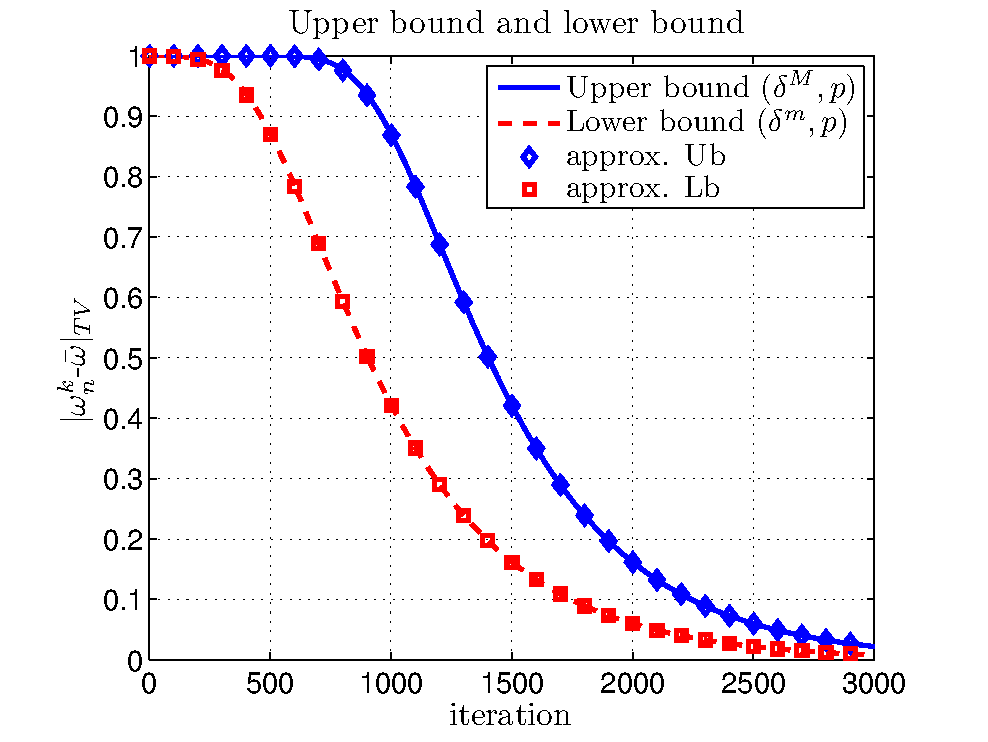
\includegraphics[width=0.5\textwidth,trim=15 0 42 0,clip]{deltaMexample2b}
  }
  \caption{\label{deltaMexample2} Left: the binomial distributions
    from the upper bound for Example~\ref{ex:exp_entries}, which
    overlap as iteration number $k$ increases, causing a sharp fall in
    the total variation. The binomials are centered at
    $p\delta_k=\frac{1}{2}+\epsilon r^k$ and $p/2$. Right: the upper
    and lower bounds of $|\omega^k-\bar{\omega}|_{TV}$ by
    Theorems~\ref{theoremub2} and~\ref{theoremlb}, as well as their
    approximations~(\ref{expub}) and~(\ref{explb}) derived from
    Theorem~\ref{theoremapproxlb}.}
\end{figure}

Examples~\ref{example:constantoega0} and~\ref{ex:exp_entries} above
show the impact of $p$ and $M$, which relate to the sum of the
stochastic symbol sequence and its largest entry. To summarize, the
total variation between the current distribution and the invariant
distribution can be characterized by its upper and lower bounds, which
correspond to $|\psi^{-1}( (\delta^m)^k )-\bar{\omega}|_{TV}$ and
$|\psi^{-1}( (\delta^M)^k )-\bar{\omega}|_{TV}$. These bounds can be
evaluated (and also approximated) and then the shape of
$|\omega-\bar{\omega}|_{TV}$ is determined.

% which
%centered at $pM$ (resp. $p\delta_{\star}^m$) and $p/2$. And so their TV can be bounded by $p$ and $M$ (resp. $\delta_{\star}^m$). Isolating the
%change of $p$ or $M$($\delta_{\star}^m$), the trajectory can be shown as the right
%plot of figure \ref{deltaMexample1} and the right plot of figure \ref{deltaMexample2}.

\subsection{Creating normal cutoffs}

\todo{MW: I changed the section title to include ``normal'', as this
  seems like the main point here?}

\todo{MW: Paragraph below rewritten, please check.}

We have shown in Example~\ref{example:constantoega0} and
Theorem~\ref{thm:mainresult1} that evolution of probability
distributions by $P$ can produce a cutoff, but we did not establish
the precise form of the limiting trajectory as it tended to a step
function. In Example~\ref{ex:exp_entries} we then showed how the
limiting trajectories can be almost exactly the normal shape seen in
Example~\ref{ex:hypbercube} and many other finite Markov chain cutoff
problems.

Here we go one step further and show how an initial distribution like
(\ref{expw0}) evolved by $P$ can have very similar
$|\omega^k-\bar{\omega}|_{TV}$ trajectory to what one sees in a cutoff
phenomenon. Now we want to take a further step to show that we can
generate a set of initial disitributions $\omega_n$, which are a
function of $n$, such that $\nu_n^k = |\omega_n^k-\bar{\omega}|_{TV}$
actually has precisely the shape~(\ref{rdwalkshape}) as $n$ goes to
infinity.

%%%%%%%%%%%%%%%%%%%%%%%%%%%%%%%%%%%%%%%%%%%%%%%%%%%%%%%%%%%%%%%%%%%%%%%%%%%%%%%%%%%%%
\begin{theorem}
  \label{thm:normal_cutoff}
  For a 1D map $S:\Lambda \to \Lambda$ with full shift symbolic
  dynamics, define the family
  $(\Omega,\bar{\omega},(\omega^k_n)_{k=0}^{\infty})_{n=1}^{\infty}$
  by the evolution $\omega^{k+1} = P \omega^k$ with the
  Perron-Frobenius operator $P$ from the initial conditions
  $\omega_n^0 \in \bar{\Gamma}$ satisfying
  \begin{align}
    \label{eqn:normal_cutoff_IC}
    \psi(\omega^0_n) =  \{.\delta_0 \delta_1 \delta_2 \cdots\},
  \end{align}
  where $\delta_i = \min\{\frac{1}{2}+\epsilon_n r_n^i,1\}$, and
  \begin{align}
    \begin{split}
      r_n &= e^{-\frac{2}{n}}\\
      \epsilon_n &= \sqrt{\frac{n(1-r_n)}{4}}.
    \end{split}
  \end{align}
  Then the family
  $(\Omega,\bar{\omega},(\omega^k_n)_{k=0}^{\infty})_{n=1}^{\infty}$
  presents a total variation-cutoff.

  Moreover, letting $k = \frac{1}{4}n\log{n}+cn$ for a fixed $c \in
  \mathbb{R}$, then as $n\to \infty$, we have
  \begin{align}
    \label{erfbound}
    % |\omega^k_n - \bar{\omega} |_{TV} \sim \erf \left(\frac{e^{-2c}}{\sqrt{8}}\right)
    \erf \left(\frac{e^{-2c-1}}{\sqrt{8}}\right)\le |\omega^k_n -
    \bar{\omega} |_{TV} \le \erf
    \left(\frac{e^{-2c}}{\sqrt{8}}\right).
  \end{align}
\end{theorem}

\begin{proof}
  From Example~\ref{example:constantoega0} we know that $|\omega^k_n -
  \bar{\omega}|_{TV}$ is bounded by (\ref{omegakbound}). As $n \to
  \infty$, we have that $\epsilon_n$ goes to $\sqrt{\frac{1}{2}}$ and $r_n$ goes to
  $1$. Letting $k> \frac{-\log(2\epsilon_n)}{r_n}$, so that $\epsilon_n
  r_n^k<1/2$, and using the results of~(\ref{expub}) and~(\ref{explb}), we have
  \begin{align}
    \erf\left( \sqrt{\frac{1}{2(1-r_n)}} \epsilon_n e^{-1} r_n^k \right)
    \le |\omega^k_n - \bar{\omega}|_{TV}
    \le \erf\left( \sqrt{\frac{1}{2(1-r_n)}} \epsilon_nr_n^k \right).
  \end{align}
  In this case these bounds are not approximations, because the
  conditions of Theorem~\ref{theoremapproxlb} are satisfied.
  Substituting the expressions for $\epsilon_n$ and $r_n$ into above
  the inequality gives
  \begin{align}
    \erf\left(\sqrt{\frac{n}{8}}e^{-\frac{2k}{n}-1}  \right)
    \le |\omega^k_n - \bar{\omega}|_{TV}
    \le  \erf\left(\sqrt{\frac{n}{8}}e^{-\frac{2k}{n}}  \right).
  \end{align}
  % Thus we have
  % \begin{align}
  %   |\omega^k_n - \bar{\omega} |_{TV} \sim \erf\left(\sqrt{\frac{n}{8}}e^{-\frac{2k}{n}}  \right)
  % \end{align}
  Letting $k = \frac{1}{4}n\log{n}+cn $ for $c\in \mathbb{R}$, and
  substituting into the above expression, we obtain the desired
  result~(\ref{erfbound}), and hence the family presents a cutoff.
\end{proof}

%%%%%%%%%%%%%%%%%%%%%%%%%%%%%%%%%%%%%%%%%%%%%%%%%%%%%%%%%%%%%%%%%%%%%%%%%%%%%%%%%%%%%%

The key idea of the above theorem is that, for a pair $(\epsilon,r)$,
we know that the stochastic symbol sequence with $\delta_i =
\frac{1}{2}+\epsilon r^i$ has a normal-shape cutoff. Hence we equate
the coefficients to find $(\epsilon_n,r_n)$ as functions of $n$ that
have the same $|\omega^k_n - \bar{\omega} |_{TV}$ as the random walk
on a $n$-dimensional hypercube problem. In this case, the $\epsilon_n$
we find is larger than $1/2$ when $n>1$, which is prohibited in the
stochastic symbol sequence (it would require $\delta_0>1$). However,
we set $\delta^i=1$ for $i<\frac{-\log(2\epsilon_n)}{r_n}$ and then
when $k> \frac{-\log(2\epsilon_n)}{r_n}$, the remaining sequence is
exponential and Theorem~\ref{theoremapproxlb} is applicable again.

Following the same procedure, we can reproduce any cutoff with a
normal shape by a family
$\{\Omega,\bar{\omega},(\omega_n^k)_{k=0}^{\infty}\}_{n=1}^{\infty}$,
where $\omega_n^{k+1} = P \omega_n^k$, and $P$ is the Perron-Frobenius
for any map $S:\Lambda \to \Lambda$ which has full shift symbolic
dynamics.

%%%%%%%%%%%%%%%%%%%%%%%%%%%%%%%%%%%%%%%%%%%%%%%%
\subsection{What causes cutoffs?}
%%%%%%%%%%%%%%%%%%%%%%%%%%%%%%%%%%%%%%%%%%%%%%%%

One way to understand the source of cutoff behavior is to regard it as
arising from systems which are composed of an increasingly large
number of almost independent events. For example, in the hypercube
random walk problem, whether each coordinate in the point's position
vector is zero or one is almost independent of the other coordinate
values, after a few iterations have elapsed. Indeed, assuming that
these processes are actually independent (corresponding to the
continuous-time random walk on a hypercube
problem~\cite{Diaconis1990}) simplifies the problem dramatically while
still giving the same cutoff behavior.

For chaotic map evolution, we have shown in
Lemma~\ref{lemma:independency} that the values of the symbols at
different positions in the symbol sequence are completely independent,
with appropriately sampled initial conditions. So this process looks
like it is composed of an infinite number of independent small
processes, and we can choose the initial probability distributions to
produce cutoff behavior. It is thus the full shift symbol dynamics of
the chaotic map evolution that is key to cutoff in this setting.

\todo{MW: I compressed a long discussion here. Please check that it is
  still correct and makes the main points.}

%As we have mentioned before, the analysis and proof of cutoffs are
%usually very hard, but to understand what causes cutoffs can be quite
%easy and we discuss it here to further explain the relation between
%the cutoff of finite Markov Chains and chaotic map mixing. Let us
%focus on the total variation-cutoff with normal shape. We claim that
%if the process is composed of many (almost) independent small
%processes, then it has the key factor to present a cutoff. To explain
%this, again we use the random walk on an $n$-dimensional hypercube as
%the example. Let $I=\{0,1\}$; the coordinate of the particle can be
%represented as a vector in $I^n$. For instance, the point starting at
%the origin is
%\begin{align*}
% x^0 = (0,0,\ldots,0).
%\end{align*}
%Each of the coordinates equals zero with probability $1$. At each
%iteration, the particle can stay fixed or choose one of the
%coordinates randomly. For this chosen coordinate, if it is $0$, it
%becomes $1$ and vice versa. Under this big process with $n$
%coordinates and $2^n$ states, we can discuss $n$ much smaller random
%processes: the value of each coordinate. All of these small processes
%are not independent of each other. For example, at iteration $1$,
%suppose we know that the first coordinate is $1$; then we immediately
%know all of the other coordinates are zeros.
%
%So even though all of these small processes are identical and easy to
%analyze, to calculate the probability of the $2^n$ states by the joint
%probability of the small processes is still not possible. Nonetheless,
%a very important fact is: they become almost independent after just
%several iterations. This is also easy to imagine: suppose $n = 1000$
%and $k = 10$; knowing that the first coordinate is $1$ is almost not
%helpful to know the value of any other coordinates. The tendency that
%these small processes have to become independent of each other is so
%strong that even if we just assume they are independent in the
%beginning, and calculate $\omega_n^k$ by the joint probability of
%these independent small processes, we get a very good approximation of
%the actual process. This simplification corresponds to the
%continuous-time random walk on a hypercube problem
%\cite{Diaconis1990}. The analysis of this problem is much easier than
%the original problem and it presents the same cutoff. Therefore, we
%can conclude that even if the original process is very complicated,
%the almost independence of the small processes is the key for the
%whole process to present a cutoff.
%
%Then how does this almost independence fit into the chaotic map
%evolution? Remember that the probability space we discuss is
%$\bar{\Gamma}$, and from Lemma \ref{lemma:independency}, when a point
%$x$ with probability distribution $\omega \in \bar{\Gamma}$ is evolved
%by the chaotic map with symbolic dynamics, $\phi(x^k)_i$ and
%$\phi(x^k)_j$ are independent of each other for all $k$ and $i\neq
%j$. So this process looks like it is composed of an infinite number of
%independent small processes. Thus we can design the exponential type
%stochastic symbol sequence to make all these small processes behave
%like the process we see in one coordinate of the hypercube and achieve
%similar total variation trajectories. It is purely the special
%property of $\omega \in \bar{\Gamma}$ for chaotic maps with symbolic
%dynamics that makes this possible. This clearly explains why we
%observe cutoffs in chaotic map evolution.

 

%%%%%%%%%%%%%%%%%%%%%%%%%%%%%%%%%%%%%%%%%%%%%%%%
%\subsection{When $\omega \notin \bar{\Gamma}$}
%%%%%%%%%%%%%%%%%%%%%%%%%%%%%%%%%%%%%%%%%%%%%%%%

%The above results are only applicable when $\omega \in \bar{\Gamma}$, and is quite restrictive. An easy extension can be made for all $\omega \in \Omega$ and are ``close'' to $\bar{\Gamma}$ in total variation distance. Given $\omega^0 \in \Omega $, suppose we can find an $\tilde{\omega}^0\in \bar{\Gamma} $ such that $|\omega^0- \tilde{\omega}^0|_{TV}$ is small, then use triangular inequality, for any $k \ge 0$
%\begin{align}
%     \left| |\tilde{\omega}^k-\bar{\omega} |_{TV}  -  |\omega^k-\tilde{\omega}^k|_{TV}\right|
%     \le |\omega^k-\bar{\omega}|_{TV}
%     \le |\tilde{\omega}^k-\bar{\omega}|_{TV} + |\omega^k-\tilde{\omega}^k|_{TV}
%\end{align}
%Total variation distance is non-increasing, thus $|\omega^k-\tilde{\omega}^k|_{TV} \le |\omega^0-\tilde{\omega}^0|_{TV} $. Let the upper and lower bounds obtained by theorem \ref{theoremub} and \ref{theoremlb} for $|\tilde{\omega}^k-\bar{\omega} |_{TV}$ be $b_l^k$ and $b_u^k$, and let $|\omega^0-\tilde{\omega}^0|_{TV} = b^0$, we have
%\begin{align}
%     |b_l^k-b^0| \le |\omega^k-\bar{\omega}|_{TV}  \le b_u^k+b^0
%\end{align}
%How do we find $\tilde{\omega}^0$ such that $|\omega^0- \tilde{\omega}^0|_{TV}$ is minimized so that the bound is tighter? The easiest way is letting $\tilde{\omega}^0 = \psi(\omega^0) $. This may not be the best fitting of $\omega^0$, however, it is believed that if $\psi(\omega^0)$ is not a good fitting of $\omega^0$, there is not much space to improved by finding another $\tilde{\omega}^0$. Again, we want to stress that the upper and lower bounds are not practically useful, but they do characterize the behavior of the convergence trajectory for a set of $\omega^0$.


%%%%%%%%%%%%%%%%%%%%%%%%%%%%%%%%%%%%%%%%%%%%%%%%%%%%%%%%%%
%%%%%%%%%%%%%%%%%%%%%%%%%%%%%%%%%%%%%%%%%%%%%%%%%%%%%%%%%%
\section{Conclusion}
\label{sec:symdynconclusion}

\todo{MW: This section is heavily reworded. Please check.}

We have proved that cutoff can be exhibited by the evolution of
probability distributions by the Perron-Frobenius operator of 1D
chaotic maps with symbolic dynamics. This connects the multistage
mixing behavior of chaotic maps with the cutoff phenomenon for finite
Markov chain evolution.

The key technique we used was a generalized symbolic dynamics, which
we called stochastic symbol sequences. This connected the evolution of
probability distributions by the Perron-Frobenius operator with the
shift map acting on stochastic symbol sequences, enabling explicit
bounds to be computed on the evolution of the total variation distance
between an evolving distribution and the invariant distribution.

We showed that a simple class of initial
conditions~(\ref{eqn:mainresult1_IC}) results in a cutoff (with the
tent map evolution of Example~\ref{ex:tentmap} as a special case), and
we also showed that a particular choice of initial
conditions~(\ref{eqn:normal_cutoff_IC}) gives cutoff trajectories with
normal shape, just as for many finite Markov chain systems.

The relationship between chaos and the cutoff phenomenon has also been
observed in numerical studies and experiments. In~\cite{numcutoff}, we
provide numerical evidence to show that the variance of functions
evolved by the Koopman operator of the diffusive standard map presents
a cutoff as the diffusion goes to zero. In~\cite{topopt}, a numerical
simulation of a chaotic mixing channel also shows cutoffs in mixing
trajectories, as do experiments for the same
problem\cite{Stroock2002}. More numerical evidence can be found in the
work of Thiffeault and Childress~\cite{Thiffeault2003-13} and Tsang et
al.~\cite{Tsang2005}, though they do not call the phenomenon
``cutoff''. These studies focus on the evolving variance of a scalar
function advected by 2D chaotic maps with small diffusion---a
different context from that explored here.  However, just as cutoff
phenomena are widespread for finite Markov Chains, we believe that
cutoffs occur in many settings for chaotic maps.

%%%%%%%%%%%%%%%%%%%%%%%%%%%%%%%%%%%%%%%%%%%%%%%%%%%%%%%%%%
%%%%%%%%%%%%%%%%%%%%%%%%%%%%%%%%%%%%%%%%%%%%%%%%%%%%%%%%%%


% References
\bibliographystyle{abbrv}
%\bibliographystyle{plain}
\bibliography{../mixingbib}




\end{document}
